

%\chapter{Drawing the Nets}
\chapter{Using Renew}
\label{ch:usage}

Renew offers a graphical, user-friendly interface for
drawing reference nets and auxiliary graphical elements.
The net editor contained within Renew is based upon a Java library
called JHotDraw \cite{Gamma98}.
The basic drawing capabilities are mainly taken over from JHotDraw,
while the multi-windowing
GUI, the net editor figures and tools, and the image figure tool
have been implemented by the Renew team.
Still, this manual covers a complete description of all drawing
and editing capabilities Renew offers.


\section{Mouse handling}

Most current computer platforms use a mouse with at least two mouse
buttons. Whenever this manual instructs you to do mouse operations,
you should use the \emph{left} mouse button. You should use the
\emph{right} mouse button only when it is especially indicated
to do so.

If your mouse has three or more buttons, the excess buttons
usually behave like the right mouse button.

Your operating system might support a special option
to switch the two mouse button, so that left handers
can operate the device more easily. This will also
switch the meanings of the mouse buttons within Renew.

Older Apple Macintosh mice have got one mouse button only.
In this case, you can press and hold the Apple key
while clicking the single mouse button, whenever
this manual commands you to press the right mouse button.
On other operating systems, too, you might be able to use
a single button mouse by pressing some control key
whenever you need access to the right mouse button.

In all cases, you can substitute right mouse clicks
by appropriate menu commands or tool selections,
but the right mouse button greatly adds to
drawing speed.

Some mouse operations react to a simultaneously held down shift or control
key.
These operations alter their behavior slightly as long as the modifier key
is pressed.
For example, a resize operation can be restricted to obtain square
dimensions as long as the control key is pressed.

If you move outside a drawing window while operating with the mouse
(i.e. while the mouse button is held down), the viewable area of the
drawing is scrolled until the drawing bounds are reached.
If you are dragging a figure or handle downward or rightward beyond the
current drawing bounds, the bounds are pushed forward until you either
release the button or move the mouse back into the window.

\section{Basic Concepts}
\label{sec:usageBasics}

When working with Renew, you edit so-called drawings.
A drawing consists of many drawing elements, called figures.
Each drawing is displayed in a separate drawing window.
Since you are expected to work on many different drawings and
thus have many different windows open at the same time, it
would consume lots of valuable desktop space to repeat
a menu bar and tool buttons in every window.
To avoid this, all commands have been grouped into one
central window, the Renew window, which contains a menubar,
a toolbar and a status line (see figure~\ref{fig:renewWindow}).
This might seen a bit unfamiliar for Mac users, but is
related with the platform independence of Java.

The shortcut \texttt{Ctrl+M} activates the central Renew
window and brings it on top of all other windows.
This key is useful if you are working with many large drawing windows,
these buried the central window and you need access to the menu bar or
tools.

\begin{figure}[htbp]
  \centerline{%
    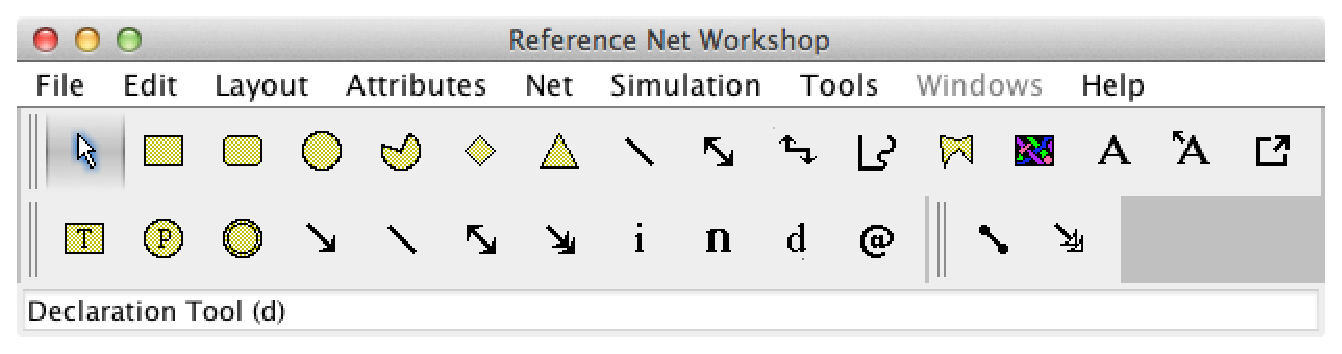
\includegraphics[scale=\screenshotscale]{RenewWin2-5.eps}%
    }
  \caption{\label{fig:renewWindow}The Renew Window}
\end{figure}%

There is always one active drawing window.
Selecting a pull-down menu invokes a command which
affects the active window, its drawing, or a selection of
figures of that drawing,
unless it has a global effect only.
Examples of menu commands are saving or loading a document
or changing attributes of figures.
The menu commands are explained in Section~\ref{sec:menuCommands}.
On the other hand, the toolbar is used for selecting a current tool.
With a tool you can create or edit certain kinds of figures in a drawing.
All tools available in the toolbar are discussed in Section~\ref{sec:tools}.
Since each tool (but the selection tool) is related to a certain type
of figures, the corresponding
figure type is also explained in that section.
To manipulate figures, handles are used. Handles are small squares or
circles that appear at special points of a figure when the figure is
selected. Dragging and (double-)clicking handles has varying effects,
depending on the kind of figure and handle.
Handles are also explained in the corresponding figure's section.

To find out how to install Renew, refer to Section~\ref{sec:install}.
You should then be able to start Renew from the command line,
just typing \texttt{renew}, or using a program icon you created,
depending on your operation system.

You can also provide some drawings' file names as command line
parameters. After typing \texttt{renew}, just provide the (path and)
name of one or more files, including the extension \texttt{.rnw}, e.g.
\begin{lstlisting}[style=xnonfloating]
  renew MyNet.rnw some/where/OtherNet.rnw
\end{lstlisting}
On start-up, Renew tries to load drawings from all specified files.
On Unix systems, you can even use
\begin{lstlisting}[style=xnonfloating]
  renew some/where/*.rnw
\end{lstlisting}
to load all drawings in a directory.

If you have a program icon that is associated correctly, your OS
usually also supports double-clicking some \texttt{.rnw} file or
using drag \& drop.

In the rare case that Renew terminates abnormally, it should leave
an autosave file for each modified net drawing. Autosave files
are typically updates every two minutes. You can detect an autosave
file by its file extension \texttt{.aut}. Whenever possible,
the filename is derived from the main drawing's file name by
removing the old name extension \texttt{.rnw} and adding
\texttt{.aut}. If such a file exists already, a random file name
of the form \texttt{rnw99999.aut} with an arbitrary number
is chosen. In order to recover an autosave file, simply rename it,
so that it receives the \texttt{.rnw} extension.

Renew also leaves \texttt{.bak} files that constitute the
last version of the file that Renew loaded. Unlike autosave files,
these files are overwritten during subsequent runs of Renew.

\section{Tools}
\label{sec:tools}

In the toolbar, several tool buttons are displayed, which can be selected by
clicking on them.

The tool buttons are grouped in two or more toolbars (depending
on the mode of Renew). When resizing the Renew window, toolbars are
wrapped according to the size of the window.
The standard toolbars are the drawing toolbar and the Petri net
toolbar.
More toolbars can show up based on the chosen formalism.

Each single toolbar can be put into its own window by clicking
at the spot on the left of the toolbar. 
Figure~\ref{fig:toolbarWindow} shows the Petri net toolbar in a
separate window.
If a toolbar window is closed, the toolbar is returned to the Renew
window.

\begin{figure}[htbp]
  \centerline{%
    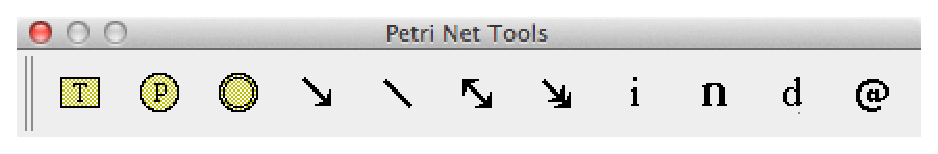
\includegraphics[scale=\screenshotscale]{Toolbar2-5.eps}%
    }
  \caption{\label{fig:toolbarWindow}The Petri Net Toolbar in its own Window}
\end{figure}%

At any point in time, exactly one tool of all toolbars is selected,
which appears pushed down.
By default, a special tool, the selection tool, is selected,
whenever the work with the current tool is finished.

If you double-click a tool button, the tool will remain active until
you explicitly select another tool or right-click on an empty spot in
the drawing.
This replaces the menu \texttt{Toggle Sticky Tools} from the
\texttt{Edit} menu.
In general, double-clicking tools is most useful during the
initial creation of nets (but there are also other, probably more
elegant ways) and the normal selection is more apt to
later modification stages.
But of course, which way to use tools also depends on your
personal preferences.

In the status line in the Renew window, a short description of the tool
is displayed if you move the mouse pointer over a tool button.
All other tools but the selection tool are used to create a certain type
of figures. Some of the tools can also be used to manipulate already existing
figures of the corresponding type.

\subsection{The Selection Tool}
\label{subsec:toolSelection}

\toolicon{SEL}
The selection tool is the most basic tool and is not related to any special
figure type.
Instead, any figure or group of figures can be selected and moved using this
tool.
If not otherwise noted, when talking about pressing a mouse button,
the primary mouse button is meant.

If the selection tool is the current tool, the following user interactions
are possible:
\begin{description}
\item[Select] By clicking on a figure, it becomes selected.
A selected figure can be recognized by its visible handles.
Depending on the type of figure, different handles appear, but in
all cases, some handles will appear. There are even non-functional
handles, which are just there to show that a figure is selected and
do not have any additional (manipulation) functionality.
If another figure is selected, the current figure becomes deselected.
To clear the current selection, click inside the drawing, but not on any
figure.
\item[Add to Selection] If the shift key is pressed while clicking on a
figure, the figure is added to or removed from the current selection,
depending on its selection status.
This way, a group of objects can be selected, which
is convenient or even required for some commands.
\item[Area Selection] If the mouse button is pressed inside a drawing, but
not inside any figure, the area selection mode is activated after a short
delay.
The starting point marks one corner of a ``rubber band'' rectangle.
While the mouse button is held down, the other corner of that rectangle can be
dragged by moving the mouse.
When the button is released, all figures that are completely inside the
rectangle area are selected.
Combining this with the ``Add to Selection'' function is possible.
\item[Inspection.] Some figures have an additional inspect
function that is invoked by double-clicking them, which displays some
additional information of the figure without modifying it.
E.g., all connected text figures (see
Section~\ref{subsubsec:toolConnectedText}:
The Connected Text Tool) select their parent during inspection.
\item[Direct Modification] Some figures have an additional direct
manipulation function that is invoked by
clicking on them with the right mouse button.
E.g., all text figures switch into edit mode.
\item[Dragging] If the mouse button is pressed inside a figure and held down,
the drag mode is activated. All figures that are currently selected are moved
until the mouse button is released.
An advanced feature of dragging is that it is possible to change a
figure's parent. For more information on this function, see
Section~\ref{subsubsec:toolConnectedText}: The Connected Text Tool.
\item[Stepwise Movement] You can use the cursor movement keys on the
keyboard to move selected figures upward, downward, leftward or
rightward in steps of one pixel.
If no figure is selected, the cursor keys scroll the viewable area of the
drawing in its window.
 By holding the shift key during cursor movement,
selected figures are moved in steps of 10 pixels.
\item[Manipulating] Depending on the kind of selected figure, handles
are displayed at special points within the figure. Using these handles, a
figure can be manipulated. The different types of handles are discussed in
Section~\ref{subsec:drawingTools} in the subsection of the corresponding
figure's tool.
\item[Open Target Location] If the control key is pressed while clicking on a
figure, the target location of the figure (if set) is opened (see 
the subsection of the target tool in Section~\ref{subsubsec:toolTarget} for details).
\end{description}

To move a single figure, it is crucial not to hit a figure's handle,
otherwise the handle's function is invoked instead of moving the
figure(s).
When more than one figure is selected, the handles of all selected
figures are shown but have no effect.
To actually use the handles, you have to select exactly one figure.
The easiest way to do so is to click on an empty spot in the drawing
and then select the figure you want to manipulate.

In Table~\ref{tab:mani} we summarize the actions of
the inspection and direct manipulation functions
for all figures. The actions associated to the different figures
are explained in more detail
in the section that documents the corresponding tool.
Some of the entries in the table refer to
the simulation mode, which will be explained in more detail
in Section~\ref{sec:simulation}.

\begin{table}
  \centerline{\begin{tabular}{l|lll}
    type of figure & double click & right click \\
    \hline
    rectangle, ellipse, \dots & select children & select/drag \\
    text & select & text edit \\
    connected text & select parent & text edit \\
    \hline
    transition & select children & attach inscription \texttt{:s()} \\
    place & select children & attach inscription \texttt{[]} \\
    virtual place & select associated place & attach inscription \texttt{[]} \\
    arc & select children & attach/edit inscription \\
    declaration & select & text edit \\
    inscription, name, label & select parent & text edit \\
    \hline
    transition instance & open binding window & fire arbitrary binding\\
    place instance & select marking & open current marking window \\
    cardinality marking & select place instance & show token marking \\
    token marking & select place instance & show cardinality marking \\
  \end{tabular}}
  \caption{Summary of selection tool operations}\label{tab:mani}
\end{table}


\subsection{Drawing Tools}
\label{subsec:drawingTools}

Renew provides several drawing tools which create and manipulate drawing
figures.
These drawing figures do not have any semantic meaning to the net simulator,
but may be used for documentation or illustration purposes.
You may lack some functions that you are used to from your favorite drawing
tool (like adjusting line width and such), but remember that Renew is a
Petri net tool, not a drawing tool in the first place.


\subsubsection{The Rectangle Tool}

\toolicon{RECT}
The rectangle tool is used for creating new rectangle figures.
Press the mouse button at the point where the first corner is
supposed to be and drag the mouse to specify the opposite corner while
holding down the mouse button.
While dragging, you can already see the rectangle's dimension and location
which is confirmed as soon as you release the mouse button.

After a new figure has been created,
the new figure is not automatically selected.
To do so, just click on the figure with the selection tool
(see Section~\ref{subsec:toolSelection}).
Now, the figure's handles appear. In the case of a rectangle or ellipse
figure, these are sizing handles which are displayed as small white
boxes at the corners of the figure.
These handles let you change the dimension (and location) of a figure
after you created it.
Depending on the position of the handle, only certain changes are
allowed. For example, the ``east'' sizing handle only allows to change
the width of a figure, while maintaining the location of the left side,
and the ``south-west'' sizing handle only lets you relocate the lower
left corner of a figure, while maintaining the location of the upper and
right side.
The ``south-east'' handle restricts itself to sizes of
  equal height and width (squares) as long as the control key is pressed.
  The control key can also be used as a modifier while you are working with
  the rectangle creation tool (and many other figure creation tools).

\newtwodotfive{  
  With the shift key pressed, the ``south-east'' handle restricts itself to constrain the proportions.
}

All newly created figures have a black outline and aquamarine as the
fill color (if there is any).
To change these attributes, use the \texttt{Attributes} menu (see
Section~\ref{subsec:menuAttributes}).
\tip{To create figures with the same attributes as an existing figure,
use copy~\&~paste (see Section~\ref{subsec:menuEdit}).}

\subsubsection{The Round Rectangle Tool}

\toolicon{RRECT}
The round rectangle tool works the same way as the rectangle tool (see above),
only that the created figure is a box with rounded corners.
A round rectangle figure has the same handles as a rectangle figure plus an
additional single round yellow handle to change the size of the curvature.
Drag this handle and change your round rectangle to anything between a
rectangle and an ellipse.

\subsubsection{The Ellipse Tool}

\toolicon{ELLIPSE}
The ellipse tool works the same way as the rectangle tool (see above),
only that ellipses are created within the given rectangle area.
An ellipse figure has the same handles as a rectangle figure.

\subsubsection{The Pie Tool}

\toolicon{PIE}

The pie tool works the same way as the rectangle tool (see above),
only that segments of ellipses are created within the given rectangle area.
A pie figure has the same handles as a rectangle figure, with two
additional ``angle'' handles that are small yellow circles.
The ``angle'' handles control start and end of the arc segment that frames
the pie.
By pressing the control key while dragging these handles around, their
movement can be restricted to steps of 15 degrees.
If a pie's fill color is set to ``none'', it displays as an open arc
segment instead of a closed pie.

\subsubsection{The Diamond Tool}

\toolicon{DIAMOND}
The diamond tool works the same way as the rectangle tool (see above),
only that diamonds are created within the given rectangle area.
A diamond figure has the same handles as a rectangle figure.

%Remark: Diamonds are a girl's best friend.

\subsubsection{The Triangle Tool}

\toolicon{TRIANGLE}
The triangle tool works the same way as the rectangle tool (see above),
only that triangles are created within the given rectangle area.
A triangle figure has the same handles as a rectangle figure, with an
additional ``turn'' handle that is a small yellow circle.
This handle lets you choose the direction the triangle points to, which
is restricted to one of the centers of the four sides or one of the four
corners.

%Remark: Triangle Man hates Particle Man.

\subsubsection{The Line Tool}

\toolicon{LINE}
The line tool produces simple lines that are not connected (see also
the next section: The Connection Tool).
Creating a line is similar to creating a rectangle:
Press the primary mouse button where the starting point is
supposed to be and drag the mouse to specify the end point while
holding down the mouse button.

The line figure has two sizing handles (small white boxes) in order
to let you change the starting and end point afterward. It also has
an {\em intermediate point\/} as described in Section~\ref{subsec:drawingTools}: 
The Connection Tool. 

A line figure has no fill color, but it respects the pen color
(see Section~\ref{subsec:menuAttributes}).


\subsubsection{The Connection Tool}
\label{subsubsec:toolConnection}

\toolicon{CONN}
This tool lets you create connections (arcs) between other figures.
A connection is like a line, except that it connects two existing figures
and is automatically adapted every time one of the connected figures changes.

Consequently, the location of pressing down the mouse button does not
specify a starting point, but a starting figure. Again, the mouse button
has to be held down while dragging the end point of the connection.
If an appropriate figure is found under the mouse button, the end point
``snaps'' into this figure's center. This figure is confirmed as the
end point figure as soon as you release the mouse button.
The connecting line always is ``cut off'' at the outline of the start
and end figure, so that it just touches their borders.

A connection can be re-connected using its green square connection handles.
Just drag one of these handles to the new start or end figure.
If you release the mouse button while the connection is not ``snapped''
into a new figure, the connection will jump back into its old position.

An advanced feature is to produce {\em intermediate points\/} (or
``pin-points'') in a connection.
When selected, connection figures show
additional {\em insert point\/} handles to create new intermediate
points in the middle of each line segment.
These are depicted as small circles with a cross (plus-sign) inside.
When you click on an insert point handle, a new location handle (see
below) is created within the given line segment and can immediately be
moved. By holding Ctrl while pressing, holding and dragging an intermediate 
point you can orient the two emerging line segments in a right angle. 

A different method to create and delete intermediate points is to use the
connection tool.
Activate the tool and click on a
point on the connecting line. Now, a new location handle (white square)
is created, which you can see the next time you select the connection figure.
This handle can be dragged to an arbitrary position.

When you hold down the control key while moving a location
handle, the intermediate point
jumps to the closest position so that the adjacent line segments
form a right angle.

You can also keep the mouse button pressed down right after clicking
on an intermediate point and drag the new handle immediately (without actually
having seen the handle itself).
If you want to get rid of a pin-point, simply
select the connection and double-click the associated handle.
Another (more complicated) way to remove intermediate points is to select
the connection tool and click on the intermediate point with the left mouse
button.

\tip{If you move two figures, a straight connection is automatically moved
with them. But if the connection has intermediate points, these stay at their
old location. Solution: Just select the connection itself additionally, and
everything will move together.}

\subsubsection{The Elbow Connection Tool}

\toolicon{OCONN}
The elbow connection tool establishes a connection between two
figures just like the connection tool.
The difference is that an elbow connection does not draw a direct
line from one figure to the other, but uses straight (horizontal
or vertical) lines only.
When you select an elbow connection, you see up to three yellow
handles which adjust the position of the horizontal and vertical
lines.
\bug{Changes to these handles are not stored.
Also, if the connected figures are close together, the decision whether
to go horizontal or vertical first is quite poor.
Since no elbow connections are needed to construct reference nets,
we do not really care about these bugs.}


\subsubsection{The Scribble Tool}

\toolicon{SCRIBBL}
The scribble tool lets you scribble in a drawing
with your mouse, just like the famous Java applet.
More precisely, a scribble figure traces the mouse movement while the
button is held down and thus defines several points, which are connected
by lines. You can also define single points by single mouse clicks.
The creation mode is ended by double-clicking at the last point or 
right-clicking in the drawing window. 
The clou about the scribble figure: After it has been
created, every single point can still be changed by dragging the
corresponding white, square handle.
To drag the whole figure, start dragging on a
line segment rather than inside a handle, or deselect the figure first
and then start dragging anywhere on a line of the figure.

\subsubsection{The Polygon Tool}

\toolicon{POLYGON}
A polygon is created analogous to a scribble figure (see above).
While you create the polygon, you can already see that the area
surrounded by the lines is filled with the fill color.
In contrast to the scribble figure, the surrounding line is closed
automatically. By intersecting the lines, you can create un-filled
areas. Like in the scribble figure, there are white, square handles
to drag every single point of the polygon figure. A point that is 
dragged to somewhere on the direct line between
its ancestor and predecessor point is removed from the polygon.
Also, there is a round, yellow handle that can be used to
turn and to scale the entire polygon figure by dragging the handle,
which looks really nice (thanks to Doug Lea).

The round, yellow handle is restricted to pure rotation
as long as the shift key is pressed and to pure scaling as long as the
control key is pressed.
The behavior of white, square point handles can be modified with the
control key similar that of location handles of connections (see above).

It can be configured how the polygon smoothness lines by removing
intermediate points.
The property \texttt{ch.ifa.draw.polygon.smoothing} can be set to the
following values (changes take effect the next time a polygon is
manipulated):
\begin{description}
  \item[alignment]
    \ This is the default behavior.
    Points are removed if they are located on a straight line between their
    adjacent points.
  \item[distances]
    \ Points are removed only if they are too close to each
    other (less than 5 pixels distance horizontally \emph{and}
    vertically).
  \item[off]
    \ No smoothing at all (no points are removed).
\end{description}


\subsubsection{The Image Tool}

\toolicon{IMAGE}
The image tool offers you the possibility to include bitmap graphics into your
drawings. When activating this tool, a file dialog box opens that lets you
choose a bitmap graphic file from your file system.
\texttt{gif} files should work on all platforms, but other formats like
\texttt{jpg}, too.
Java (and thus Renew) even supports transparent GIF images.

\bug{Be aware that the Encapsulated PostScript output does not support
transparent GIF images, but some of the other export
formats (e.g. PDF and SVG) do.
}

After you confirmed the file selection, the dialog disappears and leaves you
with two options: Either you just click somewhere in your drawing, or you drag
open an area, just like when creating a rectangle. If you just click, the image
is inserted using its original dimensions (in pixels), otherwise it is scaled
to the rectangle area specified by your drag operation.

An image figure has the same handles as a rectangle figure.

\newtwodotfive{
 With Renew 2.5 you can use drag and drop to add images. Just drag the image into the drawing editor.
}


\subsubsection{The Text Tool}
\label{subsubsec:toolText}

\toolicon{TEXT}
The text tool is used to arrange text with your graphical elements.
The first mouse click after activating the tool selects the upper left corner
of the text area and invokes a text editor.

Now you can type in any text,
including numbers, symbols, and so on. You can even use the cursor keys,
delete any characters, select some part of the text with the mouse and so on,
like in any other Java edit field.
Note that you can even type in several lines, as usual by pressing the return
or the enter key. This is why pressing return or enter does not end the edit
mode.

After you click somewhere outside of the text editing box, the text is entered
and all of the text is displayed.
If the editing box is empty at that moment (the entered text comprises white
spaces and line breaks only), the text figure is automatically removed from
the drawing.

The white box handles are just to show that a text figure is selected.
The dimension of a text figure can not be changed, as it only depends on its
text contents and font selection.
The only handle to modify a text figure is a small yellow round font sizing
handle.
It can be dragged to alter the font size, which can also be done using a menu
command (see Section~\ref{subsec:menuAttributes}). 

If you want to change the text contents of an existing text figure, just
make sure the text tool is activated and click on the text figure.
The text editor described above will appear.
Again, confirm your changes by clicking somewhere outside the editing area.

\tip{A fast way to enter text edit mode for any text figure (including connected
text, inscription, name, and declaration figures) is to right-click on these
figures. The corresponding tool is activated and the figure is put into text
edit mode immediately.}

\subsubsection{The Connected Text Tool}
\label{subsubsec:toolConnectedText}

\toolicon{ATEXT}
Connected text works exactly like normal text, except that it is connected
to some other figure, which is called its parent.

To create a connected text figure, select the connected text tool and
click on the figure that is to become the parent of the new connected text
figure. If you select a figure that cannot take a connected text figure
or if you select no figure at all, your selection is ignored.
If the figure was successfully chosen,
continue with editing text like with a normal text figure (see above).

Now, every time you move the parent figure, the connected text figure will
move with it. Only when you drag the connected text figure itself, the offset
to its parent is changed.

To verify which figure is the parent of some connected text figure,
double-click on the connected text figure, and the parent (if there
is any) is selected.

A special feature of connected text
is dragging a single connected text figure, or any special subclass like inscriptions
(see Section~\ref{subsubsec:toolInscription}: The Inscription Tool),
to a new parent.
Whenever the ``landing point'' of a connected text drag operation is another
potential parent, it is selected immediately to indicate that
instead of changing the offset to the old parent, the
targeted figure will become the new parent of the connected text figure
as soon as you release the mouse button.
If you drag the connected text figure to a location outside this new parent
again, its old parent (if there is any) is selected in the same manner,
to indicate if you let go the mouse button now, the parent will stay the same.

Note that the offset the connected text figure had to its old parent is re-established
for its new parent, so it might jump to another position after reconnection.
This is quite convenient if you moved an inscription to a
preferred offset to its parent (e.g.\ to the right-hand side of a transition),
and want to keep this offset even after connecting it to a new figure.

\subsubsection{The Target Tool}
\label{subsubsec:toolTarget}

\toolicon{TARGETTEXT}
The target tool can be used to add hyperlinks (target locations) to figures. These target locations can point to other Renew drawings, files in the file system or to a locations written as URI (e.g. a website). The target tool works like the connected text tool with the difference that the target location is only visible when edited. The target location is stored as attribute of the figure (\texttt{targetLocation}). The target locations can be opened by using the selection tool and clicking on the figure while pressing the control key (see Section~\ref{subsec:toolSelection}).



\subsection{Net Drawing Tools}

Now it is really getting interesting:
This group of tools allows you to draw Petri nets that have a
semantic meaning to the simulation engine.
Renew differentiates between a simple rectangle and a transition,
although they may look the same.
When you use the net drawing tools, some syntactic constraints
are checked immediately (see Section~\ref{sec:errors}).

\tip{Since all net element figures (transitions, places, and arcs) may have
inscriptions, Renew supports automatic inscription
%selection and
generation.
Click on a net element figure with the right mouse button,
and
%its first inscription figure is selected. If there is no inscription
%figure, a new one is created with the default inscription \texttt{x}.
a new inscription figure is created with a default inscription
depending on the type of net element.
This is especially convenient for arc inscriptions,
since these usually consist of a single variable.
Of course, in most cases, you have to change the inscription
afterward, but you do not need to use the inscription tool.
Instead, you right-click on the net element and then right-click
on the newly created inscription.
}

\subsubsection{The Transition Tool}
\label{subsubsec:toolTransition}

\toolicon{TRANS}
This tool functions almost exactly like the rectangle tool.
The differences are:
\begin{itemize}
\item Only transition figures have a semantic meaning
      to the simulator. A rectangle figure is ignored by the net
      execution engine.
\item To create a transition with a default size, after selecting the 
      transition tool, just click instead of drag. The position of the 
      click specifies the center of the newly created transition.
\item A transition figure offers an additional handle. The arc handle,
      a small blue circle in the middle of the figure, can be used to
      create new output arcs (see Section~\ref{subsubsec:toolArc}:
      The Arc Tool).
\end{itemize}

The new handle has a special behavior when you stop dragging
on figure that is not appropriate as a target for the arc.
A normal connection is deleted when there is no
appropriate end figure. However, for an arc it is quite clear what kind
of figure is supposed to be there: a place figure. And this is what happens:
Automatically, a place figure is created with its center set to the location
where you released the mouse pointer, and the newly created arc connects
the transition and the new place.

\tip{This feature offers you a very fast way to create reference nets.
Just start with a transition and use its blue arc handle to create a new arc
and the next place. Since this works for places (see below), too, you can
continue to create the next arc and transition using the arc handle of
the newly created place. If you want to reuse an existing place or transition,
just drag the arc to that figure as usual. Thus, you can create arbitrarily
complex nets without selecting any other tool!
If you combine this with the automatic inscription generation and editing
(see above), even colored nets will only take seconds to create.
}

\subsubsection{The Place Tool}

\toolicon{PLACE}
The place tool works analogously to the transition tool, only that
the arc handle (the small blue circle) creates input arcs (see
previous section). If the new arc is not released on top of an
existing transition, a new transition is created and used as the target
of the arc.

\subsubsection{The Virtual Place Tool}

\toolicon{VPLACE}
The virtual place tool is used to create virtual copies of a place.
It improves
the readability and graphical appearance of nets in which
certain places are used by many transitions.
Other Petri net tools sometimes call such a virtual copy of a place
a fusion place. If the contents of a place is needed for many
transitions, the readability of the net decreases because of
many crossing arcs. With a virtual place copy, you can draw the
same place many times, thus avoiding such crossing arcs and arcs
over long distances.

You create a virtual copy of a place by activating the virtual
place tool, then clicking on the place you want to copy (this
can also be a virtual place!) and
keeping the mouse button down while dragging the virtual place
figure to its destination location. The virtual place can be
distinguished from a normal place by the double border line
(see the graphics inside the tool button).
To find out which place a virtual place belongs to, just
double-click the virtual place.
To make this relation visible in printed versions of your nets,
you should copy the name of the place to the virtual place.
Unfortunately, the tool does not take care of the names of
virtual places automatically.
Another solution supported by the tool is to give
each group of a place and all its virtual copies a different
fill or pen color. All places belonging together
will change their colors if you change the color for
one place.

During simulation, every virtual copy of a place contains exactly
the same token multiset as its original place.
Still, it is possible to determine the marking appearance separately
for each virtual place (and the place itself)
(see Section~\ref{sec:simulation}).

\tip{A nice way to take advantage of this feature is to create
virtual copies of places with an important and extensive marking
and move these to an area outside the net. This has a similar
effect as the current marking window, but you do not get your
screen cluttered with so many windows.}

\subsubsection{The Arc Tools}
\label{subsubsec:toolArc}

The arc tool works quite the same as the connection tool (see
description in Section~\ref{subsec:drawingTools}).
The differences are, like above, that an arc has a
semantic meaning to the simulator.
A restriction coming from the Petri net structure is that
an arc always has to {\em connect one transition and one place},
not two figures of the same kind or any other figures.
The arc will not snap in on the wrong figures and disappear
if you release the mouse button over a wrong figure.
This behavior is different from when you create arcs using
the arc connection handle in places or transitions (see
Section~\ref{subsubsec:toolTransition}: The Transition Tool).

There are four arc tools for those different arc types that
are generally available:
\begin{description}
\item[Arc Tool]\hangtoolicon{ARC}
 -- This tool is used for creating {\bf input} and
{\bf output arcs}, which only have one arrow tip at their ending.
If the start figure of the connection is a place (and thus, the
end figure has to be a transition), this one-way-arc is an
input arc. If the start figure is a transition, we have an
output arc.

\item[Test Arc Tool]\hangtoolicon{LINE}
-- Here, {\bf test arcs} without any arrow tips
are created. A test
arc has no direction, as no tokens are actually moved when the
transition fires (see Section \ref{subsec:reserveAndTestArcs}).
This means it does not matter whether you start a test arc
at the place or at the transition.

\item[Reserve Arc Tool]\hangtoolicon{CONN}
-- With this tool, {\bf reserve arcs} with
arrow tips at both sides are created. Again, the direction does
not matter. For the semantics of reserve arcs, see
Section~\ref{subsec:reserveAndTestArcs}.

\item[Flexible Arc Tool]\hangtoolicon{DARC}
-- An arc with \emph{two} arrow tips on one side is created.
These {\bf flexible arcs} transport a variable number of tokens.
For the semantics of flexible arcs, see
Section~\ref{subsec:flexArcs}.
\end{description}

There are two additional arc tools that are only displayed
on request, as described in
Subsection~\ref{subsec:sequentialTools}.
\begin{description}
\item[Clear Arc Tool]\hangtoolicon{DHARC}
-- This tool is used for creating {\bf clear arcs}, which
remove all tokens from a place. You have to select the place as
the start figure and the transition as the end figure
during the creation of a clear arc. For the semantics of clear arcs, see
Section~\ref{subsec:clearArcs}.

\item[Inhibitor Arc Tool]\hangtoolicon{INHIB}
-- This tool is used for creating {\bf inhibitor arcs}, which
stop the attached transition from firing as long as certain tokens
are contained in a place. This arc features circles at both
of it end points. Again, the direction does
not matter. For the semantics of inhibitor arcs, see
Section~\ref{subsec:inhibArcs}.
\end{description}

Using the \texttt{Attributes} menu, it is possible to
change the direction of an arc after its creation.
Simply select the desired value for the attribute
\texttt{Arrow}. However, you cannot currently change ordinary
arcs to flexible arcs, or vice versa. Neither can you access
inhibitor or clear arcs this way.

Let us repeat from Section~\ref{subsec:drawingTools}
that you can create intermediate points by selecting an arc tool
before clicking on an already existing figure.
You can then drag the intermediate point to its destination.
To get rid of intermediate point, right-click the associated handles.

\subsubsection{The Inscription Tool}
\label{subsubsec:toolInscription}

\toolicon{INSCR}
Inscriptions are an important ingredient for most high-level
Petri net formalisms. An inscription is a piece of text that
is connected to a net element (place, transition, or arc).
Refer to Section~\ref{ch:reference} to find out what kind of
inscriptions are valid in our formalism. You can inscribe
types and initial markings to places. You can provide inscriptions
for arcs, in order to determine the type of tokens moved.
Transitions may carry guards, actions, uplinks, downlinks, and expressions.
Multiple transition inscriptions may be given in a single figure,
but they have to be separated by semicolons.

When editing inscription figures, you have to know that
in principle they behave like connected text figures.
This means that all functions for connected text figures
also work for inscription figures
(see Section~\ref{subsubsec:toolConnectedText}: The Connected Text Tool).
For example, to check that an inscription figure is in fact connected
to the net element you want it to be connected to,
double-click on the inscription figure.
Then, the corresponding net element should be selected.
Also, you can drag an inscription to another net element.

Again, in contrast to text figures, inscription figures have
a semantic meaning to the simulator.
By default, inscriptions are set in plain style, while labels
(text without semantic meaning) are italic.
The syntax of an inscription is checked directly after you stop
editing it (see Section~\ref{sec:errors}).
Refer to Chapter~\ref{ch:reference} for
a description of the syntax of Renew net inscriptions.

\subsubsection{The Name Tool}
\label{subsubsec:toolName}

\toolicon{NAME}
The name tool also connects text to net elements, in this case
to places and transitions only. By default, a name is set in bold
style.
The idea of a name for a place or transition is to enhance
readability of the net as well as simulation runs.
When a transition
fires, its name is printed in the simulation trace exactly like
you specified it in the name figure.
Place names are used in the simulation trace whenever tokens are removed
from or put into a place.
Also, a place's name is used in the window title of current marking windows
and a transition's name is used in the new transition binding
window (see Section~\ref{sec:simulation}).

Each place and transition should have at most one name figure connected
and each name should be unique within one net
(but the editor does not check either of these conditions).
Places and transitions without connected name figures are given
a default name like \texttt{P1}, \texttt{P2}, \dots{} and
\texttt{T1}, \texttt{T2}, \dots{}

\subsubsection{The Declaration Tool}

\toolicon{DECL}
A declaration figure is only needed if you decide to use types
(see Section~\ref{subsec:types}).
Each drawing should have at most one declaration figure.
The figure is used like a text figure, only that the text it contains
has a semantic meaning to the simulator.
The text of the declaration figure is used for import statements
as well as variable declarations (see Section~\ref{subsec:types}).

As in the case of inscriptions (see above), the content of a
declaration figure is syntax-checked as soon as you stop editing.
For an explanation of syntax errors that may occur, refer to
Section~\ref{sec:errors}.

\subsubsection{The Comment Tool}

\toolicon{COMM}
The comment tool connects comment texts to net elements. 
Comment texts have a blue text color as default and no semantic meaning for the simulator. 


% commented until final release of Maria mode
%\subsubsection{The Type Tool}
%
%\toolicon{MT}
%This tool is only available in the Maria mode as described in
%subsection~\ref{subsec:mariamode}. It creates special
%net inscriptions that are used to indicate place types and also
%place capacities in the Petri net tool Maria. These inscriptions
%are displayed in bold face italics.
%
%As in the case of inscriptions (see above), the content of a
%declaration figure is syntax-checked as soon as you stop editing.

%\subsection{Type Modeling Tools}
% hier kommen die Typhierarchie-Tools und Figures hin!

\section{Menu commands}
\label{sec:menuCommands}

This section contains a reference to Renew's menus and the
functions invoked by them.

\subsection{File}

As usual, the file menu contains every function that is needed
to load, save and export drawings.
In the following section, all menu items of the file menu are
explained.

\subsubsection{New Net Drawing (*.rnw)}

This menu invokes a function that creates a new drawing and
opens it in a drawing window in a default window size.
The new drawing is named ``untitled'' and is added to the
list of drawings in memory (see Section~\ref{subsec:menuDrawings}).

The keyboard shortcut for this function is \texttt{Ctrl+N}.

\subsubsection{New Drawing\dots}

Renew supports different kinds of
drawings (dependent on the installed plug-ins), this menu entry
opens a dialog where the type of drawing can be chosen. 
Select the appropriate drawing type in the dialog and press the
\texttt{New} button.

\subsubsection{Open Navigator}
\label{sec:navigator}

This command opens the Renew file navigator in a new window.
The navigator displays folders and their Renew-related content in a
directory tree. The navigator is shown in Figure~\ref{fig:navigator}.

The keyboard shortcut for this function is \texttt{Ctrl+Shift+N}.

\newtwodotfive{The Navigator plugin was completely reimplemented. It is now persistent and extensible. We  optionally provide some convenient extensions, such as the integration of the drawing’s diff feature (ImageNetDiff), which can now be triggered directly from the Navigator GUI. Another addition is the possibility to filter the Navigator's content and to add files and folders via drag and drop.}

\begin{wrapfigure}{l}{0.4\textwidth}
  \begin{center}
    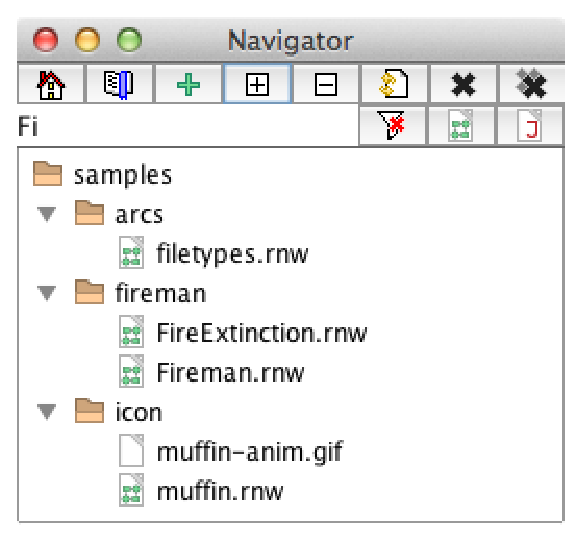
\includegraphics[scale=\screenshotscale]{Navigator2-5}
      \vspace{-30pt} % Move the caption close to the image
  \end{center}
  \caption{The Renew Navigator}
  \label{fig:navigator}
\end{wrapfigure}

\paragraph{Usage of the Navigator}
At the top of the navigator window is an icon bar with eight buttons and an additional filter bar with an input field and three additional filter buttons.
We describe these buttons and their function ``left to right''.

The \texttt{Home} button displays the home directory which defaults to the 
preconfigured files (see next paragraph) or, if there are none, to the current 
directory. 
The \texttt{NetPath} button displays all folders which are included in the netpath of Renew. This is usually empty but can be set when starting Renew or in the menu \textit{Simulation$\,\rightarrow\,$Configure Simulation$\,\rightarrow\,$Net Path}.
The \texttt{Add Folder} button opens a file choose dialog and adds the chosen directory or file to the tree.
The \texttt{Expand} button expands the complete folder structure.
The \texttt{Collapse} button collapses all nodes of the tree.
The \texttt{Refresh} button checks for new and deleted files and updates the display in the tree area.
The \texttt{Remove} button removes a single node from the tree, while the \texttt{Remove all} button removes the whole tree.

The input field can be used to filter the Navigator's content. The first button next to the input field clears the input field and the last two buttons provide predefined filters for \texttt{.rnw} and \texttt{.java} files.

The persisted state of the Navigator is saved in the file \texttt{navigator.xml} in the \texttt{.renew} subdirectory of your home directory.

\paragraph{Configuring the Navigator}
The navigator has two properties that can be configured in the usual
configuration files: \texttt{de.\allowbreak{}renew.\allowbreak{}navigator.\allowbreak{}workspace} and 
\texttt{de.\allowbreak{}renew.\allowbreak{}navigator.\allowbreak{}files\allowbreak{}At\allowbreak{}Startup}.
%
The first property defines the base directory for the navigator plugin.
It needs to be an absolute path like \texttt{/path/\allowbreak{}to/\allowbreak{}renew\renewversion{}/} or 
\texttt{c:/\allowbreak{}path/\allowbreak{}to/\allowbreak{}Renew\renewversion{}/}.
The second property is a semicolon\footnote{A semicolon has to be used even
on Unix-based systems, where paths are usually separated with the colon (:).} 
separated list of paths relative to the base directory. 
All folders and files defined in this list will be added to the tree 
area on startup.\\
Example: \texttt{MyNets;\allowbreak{}Core/\allowbreak{}samples;\allowbreak{}../\allowbreak{}../\allowbreak{}../\allowbreak{}home/\allowbreak{}renewuser/\allowbreak{}example\allowbreak{}Nets}


\subsubsection{Open URL\dots}

Renew can load drawings from a remote location
specified by a URL.
This command opens a dialog where you can type the URL and
press \texttt{OK}.
Note that Renew is not able to save drawings to URLs, it
still requires a local file name.

\subsubsection{Open Drawing\dots}

This function displays a file selector dialog that lets you select
a drawing that was saved previously.
The file selector dialog looks a little bit different depending
on the platform, but always allows you to browse the file system and
select an existing file. By pressing the OK button, the selection
is confirmed and Renew tries to load this file as a drawing.
If that does not succeed, an error message is displayed in the
application log and in the status line of the Renew window.
Otherwise, the drawing is added to the list of drawings in
memory (see Section~\ref{subsec:menuDrawings}) and opened in a new
drawing window.
The keyboard shortcut for this function is \texttt{Ctrl+O}.

The open dialog accepts the selection of multiple files.
This will result in multiple drawing windows to be opened in
the editor simultaneously.

Dependent on the set of installed plug-ins (and on your window
manager), one of several available drawing file types can be
chosen from a drop down box in the dialog.
This will restrict the display of files in the dialog.
You may override the file type filter by specifying a wildcard
pattern like \texttt{*.*} as file name and pressing
\texttt{Enter}.

\newtwodotfive{
 With Renew 2.5 you can use drag and drop to open drawings. Just drag the files into the Renew menu and tools window.
}

\subsubsection{Insert Drawing\dots}
This function opens a previously saved drawing to be inserted into the
currently focused drawing editor (Opening works like in \texttt{Open Drawing\dots{}}).
All figures which are selected before insertion are deselected. In return all
the inserted figures are selected now
which makes it easy to move them around without jamming the other figures.

\subsubsection{Save Drawing}

This function saves the active drawing (see Section~\ref{sec:usageBasics})
to a file using a textual format.
The drawing is saved to the last file name used, which is the file
it was loaded from or the file it was last saved to.
If the drawing has not been saved before, this function behaves
like \texttt{Save Drawing As\dots{}} (see below).

If there is an old version of the file, it is overwritten.
Depending on your operating system, overwriting a file might
need confirmation by the user (you).

The keyboard shortcut for this function is \texttt{Ctrl+S}.

\subsubsection{Save Drawing As\dots}

This functions is used to determine a (new) file name for a
drawing and save it in textual format (see above).

Like in \texttt{Open Drawing\dots{}}, a file selector dialog is displayed to let
you determine the (new) file name and location.
After confirming with the OK button, the specified file name
is used to store the drawing now and during future invocations
of \texttt{Save Drawing}. The name of the drawing is
set to the file name without path and file extension.
If you cancel or do not select an appropriate file name,
the drawing will neither be saved nor renamed.

Dependent on the set of installed plug-ins (and on your window
manager), one of several available drawing file types can be
chosen from a drop down box in the dialog.
The effects are similar to the effects in the \texttt{Open
Drawing} dialog explained above.
However, the list of available file types is restricted by the
type of the drawing you are going to save.

The keyboard shortcut for this function is \texttt{Ctrl+Shift+S}.

%\subsubsection{Save Drawing As Serialized\dots}
%
%This functions saves the active drawing (see Section~\ref{sec:usageBasics})
%to a file using a binary format.
%To be precise, the Java objects the drawing consists of are converted
%to a byte stream using the Java Serialization feature.
%At this point, we recommend to use the previous menu and save in
%textual format. Firstly, serialized saving has not been tested
%intensively, and secondly, it is easier to ``patch'' a textual file
%in case of changes or loading/saving errors.

\subsubsection{Save All Drawings}

This function saves all drawings that are currently in memory
(see Section~\ref{subsec:menuDrawings}).
Before this can be done, all untitled drawings have to be given
a (file) name, which is done as in \texttt{Save Drawing As\dots{}}
(see above).
If you cancel any of the save dialogues, no drawing will be saved.
If all drawings are given a proper (file) name, they are all saved.
You should invoke this function before you exit Renew (see below).

\subsubsection{Close Drawing}
\label{subsubsec:close}

Closes the active drawing window and removes the corresponding drawing
from the list of drawings in memory (see Section~\ref{subsec:menuDrawings}).
%Be careful: Unlike most other applications, Renew does not require
%a confirmation to close an unsaved drawing!
%So save first, then close!

Before doing so, Renew checks if the drawing could have been
changed (this check is a little bit pessimistic) and if so,
asks you whether to save the drawing.
You have the options to answer \texttt{Save now}, \texttt{Close},
or \texttt{Cancel}.
\texttt{Save now} tries to save the drawing.
Drawings which already have a name are saved with that name.
If the drawing is untitled, the normal save dialog appears
(see above). Here, you still have the option to cancel, which
also cancels the closing of the drawing.
If you select \texttt{Close}, the drawing is closed and all
changes since the last save are lost (or the whole drawing,
if it was still untitled).
Last but not least, you have the option to \texttt{Cancel}
closing the drawing.

The keyboard shortcut for this function is \texttt{Ctrl+W}.

\subsubsection{Close All Drawing}

Closes all opened drawing windows and removes the corresponding drawings from the list of drawings in memory. If you cancel any of the save dialogues, the process is canceled and no further drawing windows are closed.

The keyboard shortcut for this function is \texttt{Ctrl+Shift+W}.

\subsubsection{Recently saved}

The \texttt{Recently saved} menu allows you to load recently saved files.

\subsubsection{Export}

The items in the export submenu allow you to save the active drawing
in several formats for use with other applications.
The \texttt{Export} menu has three submenus.
\texttt{Export current drawing} comprises export filters for the
active drawing only.  
All these filters are available through the first menu entry
\texttt{Export current drawing (any type)}, too, where you can
choose the desired export format via a drop-down box in the file
dialog.

\texttt{Export all drawings (single file each)} provides the same
set of filters, but there they are applied to all drawings
automatically.
This results in one exported file per drawing, these files are
stored in the same location and with the same name as the respective
drawing files, but with a different extension.

\texttt{Export all drawings (merged file)} comprises export filters
that are able to merge all drawings into one file.
Since this feature must be supported by the format of the exported
file, the set of export filters in this submenu is restricted.

The export formats included in the basic Renew distribution are
listed as follows:

\paragraph{PDF}

This function produces a PDF document that contains the current drawing.
A file with the default extension of \texttt{.pdf} is generated.

The ``Renew FreeHEP Export'' plugin provides the
\texttt{de.renew.io.export.pageSize} and
\texttt{de.renew.io.export.pageOrientation} configuration properties, which
influence the page layout of generated PDF files.
Possible values for page size are: \emph{A3}, \emph{A4}, \emph{A5}, \emph{A6}, 
\emph{International}, \emph{Letter}, \emph{Legal}, \emph{Executive}, \emph{Ledger}
and \emph{BoundingBox}.
Possible values for orientation are: \emph{portrait} and \emph{landscape}.

The properties default to \emph{BoundingBox} for page size in \emph{portrait} for orientation.
However, orientation does not apply, if page size is set to \emph{BoundingBox}.

The keyboard shortcut for this function is \texttt{Ctrl+Shift+P}.

\paragraph{EPS}

If you want to include net drawings into written material,
you can use an Encapsulated Post\-script (EPS) file. The EPS file
can be used to insert graphics into other documents,
e.g.\ in LaTeX, OpenOffice, Microsoft Office, and others.
EPS files are not of a fixed page size.
Instead, their bounding box matches exactly the dimensions of the drawing.

The keyboard shortcut for this function is \texttt{Ctrl+E}.

The EPS and PDF export feature relies on the VectorGraphics
package of the FreeHEP project (see \url{java.freehep.org}). The ``Renew FreeHEP Export'' plugin provides a property for the configuration of the font handling (\texttt{de.renew.io.export.epsFontHandling}). It
can be set to \texttt{Embed}, \texttt{Shapes} or \texttt{None}.
The \texttt{Shapes} option is the default as it produces the most
similar output with respect to screen display.
However, the generated files can become rather large.
The \texttt{None} option comes close to the old Renew export behavior
without any font information included.
The \texttt{Embed} option should be the best (theoretically), but it
often produces unreadable results.

The background of drawings exported to eps can also be set to transparent 
by setting the property \texttt{de.renew.io.export.eps-transparency} to true. 

% For developers:
% The class \texttt{de.renew.util.PostScriptWriter}
% (which is a subclass of \texttt{java.awt.Graphics}
% that generates PostScript code)
% can easily be used in other applications. If you want to do so,
% please contact Frank Wienberg (see Section~\ref{ap:contact})
% to find out about capabilities and limitations of this class.
%
% \bug{The \texttt{Postscript Writer} lacks some features, so that it can not
%   always produce an exact rendering of the drawing on the screen.
%   Known missing features are:
%   transparency in GIF images,
%   transparency attribute of lines and shapes, and
%   embedding of arbitrary fonts.
%   Details are given in the respective tool explanations.}

\paragraph{PNG}

This function produces a PNG image that contains the current drawing.
A file with the default extension of \texttt{.png} is generated.
This export format differs from the previously mentioned formats since it
is pixel-oriented instead of vector-based.
The generated image has a fixed resolution that cannot be scaled without
loss of information.
The PNG export is based on the FreeHEP library.

The keyboard shortcut for this function is \texttt{Ctrl+0}.

\paragraph{XML}\label{subsec:xmlexp}
There are several export formats that use XML.
We provide experimental PNML support since Renew 2.0.
PNML stands for Petri net Markup language and has been presented
at the ICATPN'2003 in \cite{Billington2003}.
With Renew 2.2, the SVG format has been added.
With Renew 2.4, the support for the experimental XRN format provided in
previous releases has been discontinued. 

\subparagraph{PNML http://www.informatik.hu-berlin.de/top/pntd/ptNetb}
This format saves the drawing as a P/T-net, compatible with the
P/T-net type definition in a version from summer 2003.
Note that all drawing elements which are not needed to describe
the P/T-net are omitted.

\subparagraph{PNML RefNet}
This format saves the drawing as a Renew reference net.
Graphical figures without semantic meaning (e.g. those figures
produced by the drawing tool bar) are omitted.
The underlying PNML type definition is experimental, it may be
subject to changes without notice.

Please note that the PNML standard allows multiple nets to be
contained within one file.

\bug{%
  The Renew PNML export and import have been developed at a time where the
  PNML standard was still under development.
  The code has not been revised since, so that it might not comply with
  the current PNML standard.
}

\subparagraph{SVG}
This format exports the complete graphical information of a drawing into an
SVG image file which can be displayed by many modern web browsers.
Petri net semantics are not retained.
The SVG export is based on the FreeHEP library.

\paragraph{Woflan}

Woflan (see~\cite{Woflan98})
is a Workflow Analysis tool that checks if a Petri net
conforms to some restrictions that make sense for Workflows.
As Woflan only handles single, non-colored Petri nets without
synchronizations, only the structure of the active window's net
is exported. Still, if you have the Woflan tool, it makes sense to check
Renew workflow models for severe modeling errors in their structure.

For the time being, the initial place of the workflow net must
carry the name \texttt{pinit}. Otherwise, a place with this name
(but without any connected arcs) will be generated in the
exported net.

% commented until final release of Maria mode
%\paragraph{to Maria\dots}\label{subsec:mariaexp}
%
%Exports the active drawing in the Maria format.
%This command is only available in the Maria
%mode as described in subsection~\ref{subsec:mariamode}.

\paragraph{Shadow Net System}\label{subsec:expshadow}

A \emph{shadow net system} can comprise one or more nets
which can be used by the non-graphical simulator (see
section~\ref{sec:simulationServer}), the net loader or other
tools.
Only the
semantic information is contained in the shadows, but not
the visual appearance.

The current formalism (see section~\ref{subsec:formalismgui}) and the
configuration of simulation traces for individual net elements (see
section~\ref{subsubsec:trace}) will be stored within the shadow net
system.

\subparagraph{As merged file}
A shadow net system that contains all nets needed for a
simulation can be generated by the \texttt{N to 1} entry in the
\texttt{Export all drawings (merged file)} menu.
Before exporting a collection of nets to the shadow simulator, it
is recommended to do a syntax check on the net. 
Although any syntax errors in the nets will be detected before the
start of a non-graphical simulation, fixing these errors requires the
editor.

The current formalism (see section~\ref{subsec:formalismgui}) and the
configuration of simulation traces for individual net elements (see
section~\ref{subsubsec:trace}) will be stored within the shadow net
system.

\subparagraph{As single file each}
These files are well suited for the net
loading mechanism described in subsection \ref{subsec:netLoading}.

The command does not require any additional interaction, all file
names are derived from the corresponding drawing files. If a
drawing has not been assigned a file name, it is skipped during
the export.

\subsubsection{Import}

The items in the import menu allow you to load drawings from
different file formats.

\paragraph{import (any type)}
The first entry of the Menu combines all import filters into 
one dialog where you can choose the desired format from a
drop-down box.
For window managers where this drop-down box is not available,
the separate menu entries are still available.

\paragraph{XML}
Analogous to the export features described in
subsection~\ref{subsec:xmlexp}, Renew provides
the PNML format as import filters.

%\subparagraph{XML}
%Imports a file in the obsolete XML format of Renew 1.6.
%Whenever possible, the graphical and semantic information
%is restored from the file.
%
%Note again that you will not be able to import an
%XML file of a different Renew version with this command!
%
%This feature has been cannot be used anymore. Its support
%has been discontinued.

\subparagraph{PNML}
Tries to import a file in PNML format.
The filter automatically guesses the net type used in the PNML
file.
It tries to extract as much graphical and semantic information
as possible from the file.

\paragraph{Shadow Net System}
Lets you import a previously exported (or automatically
generated) shadow net system (see above).

Since a shadow net system does not contain any graphical
information,
the places, transitions, arcs, and inscriptions are
located in a rather unreadable manner.
Thus, this function only makes sense for shadow net systems
automatically generated by other tools.
After importing, it is of course also possible to edit all
nodes and inscriptions in a normal fashion.
An automatic graph layout function that can
ease the task of making an imported net readable
is described in Subsection~\ref{subsubsec:netlayout}.


\subsubsection{Print\dots}

The print menu invokes a platform dependent print dialog and lets you
make hardcopies of the active drawing. Using the Java standard print
system, though, the quality of the printer output is usually very
poor. In that case, we encourage to use the EPS or PDF export instead and print with an external tool.

The keyboard shortcut for this function is \texttt{Ctrl+P}.


\subsubsection{Exit}

Tells Renew to terminate. 
All drawings are closed as if you closed them manually,
which means that now Renew asks you about saving
changed drawings (see Subsection~\ref{subsubsec:close}).

Due to the introduction of the plug-in system, other plug-ins might
still be active when the editor is closed.
With respect to the simulator plug-in, the editor asks you for
confirmation to terminate a running simulation (if there is any).
If you choose \texttt{No}, then the non-graphical simulation of
Renew will continue.

To enforce that the whole plug-in system is shut down when you
close the editor, you can configure the property
\texttt{de.renew.gui.shutdownOnClose} (see
Subsection~\ref{subsec:systemExit} for details).

\subsection{Edit}
\label{subsec:menuEdit}

The Edit menu contains functions to insert, remove and group
figures and to change a figure's Z-order.
Details can be found in the following sections.


\subsubsection{Undo, Redo}
Up to ten modifications to each drawing can be undone step by
step. The effect of an undo can be undone by the redo command. The keyboard shortcut for undo is \texttt{Ctrl+Z} and for redo it is \texttt{Ctrl+Y}.

\subsubsection{Cut, Copy, Paste}

This function group offers the typical clipboard interactions.
Cut and Copy relate to the current selection in the active drawing
window (see Section~\ref{sec:usageBasics}).
Thus, these functions are only available if there is a
current selection.

{\bf Cut} puts all selected figures into the clipboard and removes
them from the drawing. The keyboard shortcut for Cut is \texttt{Ctrl+X}.

{\bf Copy} puts all selected figures into the clipboard, but they
also remain in the drawing. The keyboard shortcut for Copy is \texttt{Ctrl+C}.

{\bf Paste} inserts the current clipboard contents into the active
drawing. The upper left corner of the object or group of objects is
placed at the coordinates of the last mouse click.
The keyboard shortcut for Paste is \texttt{Ctrl+V}.

Note that due to restrictions of Java, Renew's clipboard does not
interact with your operating system's clipboard.

The current selection is automatically extended
to include all referenced figures before copying to the clipboard.
If for example you select an arc inscription and invoke copy and
then paste, the arc, the start figure, and the end figure of the arc
will also be copied. This is sometimes not what you intended to do,
but you can easily move the copied arc inscription to the original
arc (see Section~\ref{subsubsec:toolConnectedText}) and remove the
other duplicated figures.
Of course, cut only removes the figures which were originally selected.

\tip{The better alternative to copy inscriptions is to mark and copy
  the text of the inscription when you are in text edit mode
  (\texttt{Ctrl+C}, unfortunately, this does not work on all Unix
  platforms).
  Then, create a new inscription by right-clicking the net element.
  Edit the new inscription by right-clicking it and paste the copied
  text by pressing \texttt{Ctrl+V}.
}


%Bug fixed
%\bug{Connection figures should only be copied and pasted together with
%the figures they connect. Otherwise, pasting will create a copy of the
%connection figure that is not associated correctly to its start and end figure.
%To correct this, drag both connection handles and release them on other
%or even on the same figures.
%The same holds for connected text figures. After pasting, a connected text
%figure has to be assigned to a new parent like described in
%Section~\ref{subsubsec:toolConnectedText}: The Connected Text Tool.
%}


\subsubsection{Duplicate}

Duplicate works like Copy followed by Paste (see previous Section),
where the paste coordinates are not depending on the last mouse
click, but are just a small offset to the right and down from the
position of the original selection.
%Bug fixed:
%Mind the bug described above for the paste function!

The keyboard shortcut for Duplicate is \texttt{Ctrl+D}.

\subsubsection{Delete}

Removes the selected figures from the active drawing.
Note that if a figure is removed, all its connected text
figures and connection figures are also deleted.

The keyboard shortcut for Delete is the backspace and/or the delete key
(depending on the platform).

\subsubsection{Search, Search \& Replace}

\textbf{Search} looks for a match or substring-match of an
user given search string in all textfields of all loaded nets. Search is
case sensitive. After an occurrence of the search string is found the next
can be found by pressing the \texttt{search} button again. 
Changes on the search string start
a new search.
The keyboard shortcut for this function is \texttt{Ctrl+F}.

\textbf{Search \& Replace} gives the opportunity to replace any found
search string with a replace string. Each replacement is prompted and has
to be confirmed by the user.  Changes on the replace string start a
new search.
The keyboard shortcut for this function is \texttt{Ctrl+G}.

%TODO{Ctrl+G does not work for me, need Shift additionally.\\}

The search window allows you to select, whether the search should
be case sensitive and whether the search shall include all drawings or only
the active one.


\subsubsection{Group, Ungroup}

You can create a group of all currently selected figures in the active
drawing. A group is actually a new figure, which consists of all the
selected figures. You can even group a single figure, which does not
really make sense unless you want to prevent resizing of this figure.
From now on, the figures inside the group can only be moved, deleted,
etc. together, until you ``ungroup'' the group of figures again.
To release a group, one or more groups have to be selected.
Then, select the Ungroup menu, and all group participants are single
figures again (which are all selected).

\subsubsection{Select All}

Commands that allow selection or deselection
of large sets of nodes allow the user
to select groups of logically related net elements together.
For selecting locally related net elements or individual net
elements see Subsection~\ref{subsec:toolSelection}.

Using the select all command, all figures of a drawing are selected.
This is useful when you want to move all the net elements
to a different place. This command works even for figures that are located
off-screen.
The keyboard shortcut for this function is \texttt{Ctrl+A}.

\subsubsection{Invert Selection}

Inverts the selection of the drawing: All selected net elements will be
removed from the selection, whereas all the other net elements will be
selected.

\subsubsection{Select}

This menu hierarchy is used to select all nodes of a certain type.
E.g., it offers the possibility to select all transitions,
or all arcs, or all inscriptions that are attached to places.

This command comes in handy when you want to set attributes like
color or font size for all figures of a certain type.

\subsubsection{Add To Selection}

This command is similar to the select command, but it does not clear
the selection before it selects the net elements, thereby achieving
a union of the selection sets.

This command is especially useful when you want to select
a combination of net elements that is naturally covered
by the selection command itself. E.g., you can select all transitions
and then add all inscriptions of transitions to the selection.

\subsubsection{Remove From Selection}

This command is the opposite of the add-to-selection command.
It removes certain figures from the selection, but leaves
the selection state of the remaining figures unchanged.

This command can be used to select all figures, but \emph{not}
the transitions or \emph{not} the arcs.

\subsubsection{Restrict Selection}

Sometimes you want to select a certain type of net elements
inside a certain area. In this case, the restrict command
allows you to select the entire area as described in
Subsection~\ref{subsec:toolSelection}, but to restrict the selection
to a certain type of figures afterward.

The remove-from-selection command can be used instead of
this command, if you want to specify the figures to drop from
the selection instead of the figures to keep in the selection.

%\subsubsection{Toggle Sticky Tools}
%removed in Renew 1.4
%
% Selecting this menu toggles the Sticky Tools mode of Renew.
% By default, a tool will deactivate itself after the completion
% of a single task. Afterward, the selection tool will be
% reenabled. In Sticky Tools mode all tools will remain
% activated until you choose another tool explicitly.

% In general, Sticky Tools mode is most useful during the
% initial creation of nets and the default mode is more apt to
% later modification stages.
% But of course, which mode to use also depends on your
% personal preferences.

\subsection{Layout}
\label{subsubsec:netlayout}

The \texttt{Layout} menu allows to snap figures to a grid, to
align a figure's position according to other figures, to change the
Z-order of figures and to layout graphs automatically.

\subsubsection{Toggle Snap to Grid}

Selecting this menu toggles the Snap to Grid mode of Renew.
This grid is not absolute referring to the page, but
means that when the grid is active, figures can only be
placed to grid positions and moved by certain offsets.
Because the editor considers offsets while moving (not absolute
coordinates), figures should be aligned first (see below) and
then moved in grid mode.
\newtwodotfive{
The grid function is also very
basic, but the grid density is now customizable. 
Set the option \texttt{ch.ifa.draw.grid.size} to the desired value in
your preferences. Default is \emph{5} pixel. This preference is
dynamic, i.e. can be set at runtime. Effects take place during next
execution of command.  The grid can now also be set as the default
behavior for drawing views. Set the \texttt{ch.ifa.draw.grid.default}
property to \emph{true} (default \emph{false}).}

\subsubsection{Align}

The commands in this menu align the selected figures.
The figure selected first is the reference figure which
determines the coordinates for all others.

\paragraph{Lefts, Centers, Rights.}
These commands align the figure's $x$-coordinates, i.e.\ they move them
horizontally.
\texttt{Lefts} sets the left-hand side of all selected figures to
the $x$-coordinate of the left side of the figure that
was selected first, \texttt{Rights} does the same for the
right-hand side.
\texttt{Centers} takes into account the width of
each figure and places all figures so that their $x$-center
is below the reference figure's $x$-center.

The keyboard shortcut for aligning middles is \texttt{Ctrl+}{\textbackslash} 
(the backslash character).
\bug{%
The shortcut works only on an English keyboard layout, where the 
keys for the shortcut can be typed directly, i.e. without additional 
modifiers like Shift.%
}

\paragraph{Tops, Middles, Bottoms.}
These commands work exactly like the commands in the previous
paragraph, except that the $y$-coor\-dinate is changed.
Thus, figures are moved vertically in order to be aligned
with their tops, middles, or bottoms.

The keyboard shortcut for aligning middles is \texttt{Ctrl+-} (the minus sign).

\subsubsection{Spread}

The items of this menu spread the selected figures equidistantly.
The two outermost figures that are selected stay at their previous location
while all other selected figures are repositioned.
The order of the figures (left-to-right, top-to-bottom or
diagonal) remains unchanged.
To use the spread commands, you must have selected at least three
figures.

\paragraph{Lefts, Centers, Rights, Distances.}
Here we spread the figures by modifying their $x$-coordinates. The
$y$-coordinate remains unchanged.
\texttt{Lefts} arranges the figures in a way that the
$x$-coordinates of their left borders are distributed equally.
\texttt{Rights} does the same with respect to the figure's right
borders, \texttt{Centers} with respect to each figure's center
point.
\texttt{Distances} arranges the figures in a way that the space
in between of each pair of neighboring figures will have the same
width.
The differences between the four commands will only be visible
when figures of different sizes are selected.

\paragraph{Tops, Middles, Bottoms, Distances.}
These functions work exactly like the functions in the previous
paragraph, except that the $y$-coordinate is changed.
Thus, the figures are moved vertically to equal the distances of
their tops, middles, bottoms or borders.

\paragraph{Diagonal.}
This command spreads the figures in both directions, horizontally and
vertically.
All figures are treated with respect to their center point.
First of all, a virtual line is drawn from the outermost figure (in
relation to the center of the bounding box of all selected
figures) to the figure most apart from the outermost one.
Afterward, all other figures are moved onto that line with equal distances
between their center points.
The order of the figures on the line is determined by the
order of the orthogonal projections of their original location onto the
virtual line.

\subsubsection{Send to Back, Bring to Front}

The figures in a drawing have a so-called Z-order that determines
the sequence in which the figures are drawn.
If a figure is drawn early, other figures may cover it partially
or totally.

To change the Z-order of figures, the functions \texttt{Send to Back}
and \texttt{Bring to Front} are available. \texttt{Send to Back}
puts the selected figure(s) at the beginning of the figure list and
\texttt{Bring to Front} puts it/them at the end, with the result
explained above.

\tip{Sometimes, certain figures can not be reached to select and modify
them. Using these functions it is possible to temporarily move
the covering figure to the back, select the desired figures, and
move the figure to the front again.
Another option in cases like this one is to use Area Selection
(see Section~\ref{subsec:toolSelection}).
}


\subsubsection{Figure size}

These two commands set the size of figures.
The function \texttt{copy within selection} sets
the size of all selected figures to the size of
the figure that was selected first.
The command \texttt{reset to default} resets the selected
figure's sizes to their figure type specific default. As there
are defaults specified only for net element figures, the command
will not have any effect on ordinary drawing figures.



\subsubsection{Automatic Net Layout\dots}

Especially for automatically generated nets, it is nice to
have an automatic layout of the net graph, so that one gets
at least a rough overview of the structure of the net.

This menu entry start an automatic net layout on the
current drawing.
While this mode is active, the nodes of the net are moved according
to certain rules that are to some extend inspired by
physical forces acting on a mesh of springs.
\begin{itemize}
\item Arcs have a certain optimal length that is dependent
  on the size of the adjacent nodes. They will act as springs.
\item Arcs feel a torque whenever they are not horizontally
  or vertically oriented. The torque works toward these optimal
  positions.
\item Nodes feel a repulsive force from each other until
  a certain distance is reached where this force disappears entirely.
\item Nodes feel friction, i.e., the motion that was caused
  by the forces mentioned before continually slows down unless the force
  is still applied and compensates the friction.
\item Nodes that would move out of the upper or left border
  are pushed back into the viewable area of the drawing.
\end{itemize}
These rules will not produce the nicest net graph in many cases,
but they can ease the early stages of the layout considerably.
They might also be used to maintain a layout during early prototyping
phases when the structure of a net changes constantly.

In order to improve the layout of the graph, a special window
pops up that allows you to control some parameters or the physical model
using sliders. The first slider controls the length of the
springs. Some diagrams tend to clump together too much, which might
can be a reason to raise this value. On the other hand, the
spring might be too rigid, not allowing some springs to stretch to
their optimal length. In that case, you can control the rigidity of
the spring with the second slider.

The repelling force acts only up to a certain distance.
By default, the force is quite far reaching and establishes
a nice global spreading. But you may want to reduce this force's
maximum distance in order exclude only overlapping nodes.
In that case, it may also be good idea to increase the repulsion strength.

The torque strength controls whether the arcs are supposed to be
very strictly horizontal or vertical. Initially, this force might
actually inhibit the progress toward to optimal layout, but in the
end it helps to get a nice net. Try to vary this slider's position
during the layout for optimal results.

Lastly, the friction slider may be lowered, so that the motion is
faster overall. Use this slider with care, because the layout
algorithm may become unstable for very low friction values and
convergence to an equilibrium might actually slow down due to
oscillations. The optimal value depends heavily on the topology of the net.
If you feel that you cannot set some force's strength high enough,
consider lowering the other forces, and also lowering the friction
a little.

\tip{Even while the graph is changed automatically, you can still
grab a node with the selection tool and move it to a desired position.
Of course, it might fall back into the old position due to the
acting forces, but your action might establish a topologically
different situation where the forces act toward a different
equilibrium. This is especially useful when you have selected high torque
and rigid springs, but low or no repulsion.
}

After you are satisfied with the graph, switch off the layout mode.
If you add or remove nodes or arcs during the layout procedure,
you have to restart the net layout algorithm, before these changes
affect the layout algorithm. Note that the start of a layout procedure
always affects the current drawing, not the drawing that was previously
used for layout.

\subsubsection{Location}

Using this menu you can declare the currently selected
figures as either fixed or dynamic. Dynamic nodes participate in the
automatic layout as usual, which is the default.
On the other hand, fixed nodes still exert forces
upon other nodes, but they are rigidly glued to their position
and move only if the user moves them.

By fixing the location of some nodes, you can select a preferred
direction or specify the basic shape of the net while leaving the details
to the layout algorithm.


\subsection{Attributes}
\label{subsec:menuAttributes}

This menu helps you to change a figure's attributes after its
creation. If several figures are selected, the attribute is
changed for all figures that support that attribute.
If you try to change an attribute that some selected figures do
not support (e.g.\ font size for rectangles), nothing
is changed for that figures, but the change is still applied
to the other figures.

\subsubsection{Fill Color}

The fill color attribute determines the color of the inner
area of a figure. All figures but the line-based figures like
connection, arc, etc.\ offer this attribute.
The values for this attribute could be any RGB-color, but the
user interface only offers 14 predefined colors from which
you can choose. The default fill color is Aquamarine except for
text figures, where it is None.

When you choose \texttt{other\dots} at the end of the list of colors, you
get a full-featured color chooser dialog that provides multiple ways to
define any color.
There are four buttons at the bottom of the dialog:

\begin{description}
\item[Apply] applies the currently chosen color to selected figures.
\item[Update] chooses the color of a selected figure and makes it the
  current color in the dialog.
\item[OK] closes the dialog and applies the currently chosen color to
  selected figures.
\item[Cancel] closes the dialog.
\end{description}
\tip{The dialog can be used to copy color attributes between figures by a
  sequence of \texttt{Update} and \texttt{Apply} actions.  Similar dialogues
  are provided for other attributes like pen color, text color, font and
  font size.}

\subsubsection{Opaqueness}
The opaqueness attribute determines the transparency of the inner area of a figure, 
of the pen color or of the font. 
Each attribute \texttt{Fill Color}, \texttt{Pen Color} and \texttt{Font} has its own 
opaqueness menu that is located right below each menu entry.
The visibility of each item can be set in values ranging from 0\% (invisible) 
to 100\% (opaque).%

\bug{The transparency attribute is ignored in EPS export.  
  However, transparencies are printed correctly using the Print dialog and
  in the PDF, SVG and PNG export formats.}

\subsubsection{Pen Color}

The pen color attribute is used for all lines that are drawn.
All figures but the image figure support this attribute.
Note that the pen color does not change a text figure's
text color (see below), but the color of a rectangle frame
that is drawn around the text.
Again, choose the desired color from the given list.
The default pen color is black, except for text figures, where
it is None (i.e.\ transparent).
The \texttt{other\dots} entry at the end of the list of colors opens a
full-featured color chooser dialog as described under \texttt{Fill color}.

\subsubsection{Visibility}

The visibility attribute can be used for all types of figures.
A figure marked as invisible is still part of the drawing, but
it will not be displayed. As it is not visible, it cannot be
selected by the mouse any more, but the select commands from
the menus \texttt{Edit} or \texttt{Net} will still include the
figure when appropriate.
This feature is useful especially in combination with the
\texttt{Associate highlight} command from the net menu. The
invisible figure will appear in the instance drawing while it
is highlighted.

\subsubsection{Arrow}

This attribute is only valid for the connection and the
arc figure and offers four possibilities of arrow tip
appearance: \texttt{None}, \texttt{at Start}, \texttt{at End},
or \texttt{at Both} ends of the line.
If the figure is an arc, its semantics are changed accordingly.

\subsubsection{Arrow shape}
This attribute is valid only for lines or connection figures.
The style of arrow tips can be changed to one of four shapes,
which are usually used to mark different semantics of arcs in
Renew.
But as it is currently not possible to change the arc semantics
in accordance to the arrow tip shape, this attribute will not
have any effect on arc figures.

\subsubsection{Line Style}

Every line possesses a line style, which can be chosen out of
the options \texttt{normal}, \texttt{dotted}, \texttt{dashed},
\texttt{medium dashed}, \texttt{long dashed} or
\texttt{dash-dotted}.
Lines are typically created as solid, normal lines.

It is also possible to define your own line style: After
choosing the option \texttt{other\dots{}}, you can enter any
custom line style in a non-modal dialog.
The dialog has four buttons \texttt{Apply}, \texttt{Update}, \texttt{OK}
and \texttt{Cancel} that work similar as in the \texttt{Fill color} dialog
(see above).

A custom line style consists of a space-separated sequence of numbers.
The first number of the sequence determines the length (in
pixels) of the first dash. The second number is interpreted as
the length of the gap after the first dash. The third number
determines the second dash's length, then the next gap's length
follows and so on.

The sequence must consist of an even number of numbers. There is
only one exception: A single number can be used for a simple dashed
line where dashes and gaps are of the same length.
The normal solid line style can be set by applying an empty sequence.
\begin{tabbing}
\texttt{medium dashed}\quad\quad\=''7 3 1 3''\quad\quad\=\kill
Some examples from our predefined line styles:\\
\texttt{dashed} \> ``10'' \> \begin{picture}(90,1)(0,-4)
  \put(0,0){\line(1,0){10}}
  \put(20,0){\line(1,0){10}}
  \put(40,0){\line(1,0){10}}
  \put(60,0){\line(1,0){10}}
  \put(80,0){\line(1,0){10}}
\end{picture} \\
\texttt{medium dashed} \> ``15 10'' \> \begin{picture}(90,1)(0,-4)
  \put(0,0){\line(1,0){15}}
  \put(25,0){\line(1,0){15}}
  \put(50,0){\line(1,0){15}}
  \put(75,0){\line(1,0){15}}
\end{picture} \\
\texttt{dash-dotted} \> ``7 3 1 3'' \> \begin{picture}(90,1)(0,-4)
  \put(0,0){\line(1,0){7}}
  \put(10,0){\line(1,0){1}}
  \put(14,0){\line(1,0){7}}
  \put(24,0){\line(1,0){1}}
  \put(28,0){\line(1,0){7}}
  \put(38,0){\line(1,0){1}}
  \put(42,0){\line(1,0){7}}
  \put(52,0){\line(1,0){1}}
  \put(56,0){\line(1,0){7}}
  \put(66,0){\line(1,0){1}}
  \put(70,0){\line(1,0){7}}
  \put(80,0){\line(1,0){1}}
  \put(84,0){\line(1,0){6}}
\end{picture}
\end{tabbing}

Line styles can not only be applied to lines, connections and scribble
figures, but also to rectangles, ellipses, polygons, transitions, places
and other closed shapes.

\subsubsection{Line Shape}
With this attribute a \texttt{straight}
line can be changed to a \texttt{B-Spline} and vice
versa. Every linetype can be changed to a B-spline. But
these lines retain their other like handles and behavior.
If this conversion is applied, there are more attributes offered to
influence the bspline algorithm:
\begin{description}
\item[\texttt{standard}] This works as a reset
to standard settings with a degree of 2 and a segment size of 15.
\item[\texttt{Segments}] This is used to
change the number of segments to smooth the edges.
\item[\texttt{Degree}] The lower the number, the closer
 the line sticks to the handles. 2 creates maximally curved line.
The degree depends on the number of handles and is only effective
if the choice is not larger than the number of handles plus one.
\end{description}

\subsubsection{Round corners}
This attribute influences the behavior of round rectangles
when they are scaled.
When set to \texttt{fixed radius}, the size of the curvature
will remain unchanged regardless of the scaling of the figure.
Nevertheless, an explicit modification of the radius is still
possible by using the special yellow handle. This is the
default, which was exclusively used in previous releases of Renew.

The setting \texttt{scale with size} will adapt the curvature
size when the rectangle is scaled, so that the proportion of
the rectangle used for the curvature remains the same.

\subsubsection{Font}

Only applicable to text-based figures, this attribute
sets the font for the complete text of this text figure.
Not all fonts are available on all platforms.
It is not possible to use several fonts inside one text figure
(but still, this is a graph editor, not a word processor or
DTP application).
The \texttt{other\dots} entry at the end of the list of colors opens a
font selection dialog that works like the color dialog described 
under \texttt{Fill color}.  
The font selection dialog includes other font attributes like the size or
italic and bold style options.

\emph{Caution:} If you use non-standard fonts, the text will show
up differently on systems where the fonts are not installed.

% \bug{
%   Any non-standard font will cause problems with Postscript or EPS
%   export of the drawing.
%   The export filter is not capable to embed fonts.
%   If font names contain spaces, the postscript code becomes faulty.
% }

\subsubsection{Font Size}

Only for text-based figures, select one of the predefined font sizes
given in point with this menu.
The \texttt{other\dots} entry at the end of the list opens a dialog where you
can enter any number as size.
The dialog has four buttons \texttt{Apply}, \texttt{Update}, \texttt{OK}
and \texttt{Cancel} that work similar as in the \texttt{Fill color} dialog
(see above).

\subsubsection{Font Style}

Available font styles (again, only for text-based figures) are
Italic and Bold. If you select a style, it is toggled in the selected
text figure(s), i.e.\ added or removed. Thus, you can even combine
italic and bold style. To reset the text style to normal, select
Plain.

\subsubsection{Text alignment}
The direction of text justification can be configured by this
attribute. This will affect the alignment of lines in text figures with
multiple lines as well as the direction of growth or shrinking
when a text changes its width due to a change in its text length.
By default, inscriptions and other connected text is centered at
the parent figure while other text figures are left-aligned.

\subsubsection{Text Color}

The text color attribute is only applicable to text-based figures and
sets the color of the text (sic!). This is independent of the pen and
fill color. The default text color is (of course) black.
The \texttt{other\dots} entry at the end of the list of colors opens a
full-featured color chooser dialog as described under \texttt{Fill color}.

\subsubsection{Text Type}

This attribute is quite nice to debug your reference nets quickly.
The text type determines if and what semantic meaning a text
figure has for the simulator.

If a text figure is a \texttt{Label}, it has no semantic meaning at
all. If it is a \texttt{Inscription}, it is used for the simulation
(see Section~\ref{subsubsec:toolInscription}: The Inscription Tool).
A \texttt{Name} text type does not change the simulation, but makes
the log more readable (see Section~\ref{subsubsec:toolName}: The Name Tool).

\tip{It is quite convenient to ``switch off'' certain inscriptions by
converting them to labels if you suspect them causing some problems.
This way, you can easily re-activate them by converting them back
to inscriptions.
}

You might also want to have certain inscriptions appear as transition
names during the simulation. You can achieve this by duplicating the
inscription figure, dragging the duplicate to the transition (see
Section~\ref{subsubsec:toolConnectedText}: The Connected Text Tool)
and changing the duplicate's text type to \texttt{Name}.


\subsection{Net}
\label{sec:net-menu}
This menu offers commands that are useful for nets only.
You can semantically modify figures in a drawing, check
the active drawing for problems, or configure the
graphical simulation feedback for net elements.

\subsubsection{Split transition/place}
This command provides a simple way to refine net
elements by splitting a single transition or place into two.

If a transition is split the old transition is connected to a
newly created place. This place, in turn, is connected to a
newly created transition. The inbound arcs of the old
transition remain unchanged, the outbound arcs are reconnected
to the new transition. Reserve arcs are split into an inbound
and an outbound arc, which are handled respectively.

If a place is split it will be extended by a new transition and
a new place. The connected arcs are treated in the same manner
as described above (outbound arcs are reconnected to the new
place).

\subsubsection{Coarsen subnet}
This command coarsens place-bounded or transition-bounded subnets.
It is only available if a place-bounded or transition-bounded
subset of figures is selected within the drawing.

On execution,
if the selected subset is place-bounded,
all places are merged into one and all transitions are removed.
The inscriptions of the removed places are attached to the single
remaining place.
All arcs entering or leaving the selected subnet are
reconnected to this place, too.

If the selected subset is transition-bounded, transitions are merged and
places are removed, respectively.



\subsubsection{Trace}
\label{subsubsec:trace}

This menu and the next two are realized as figure attributes
that can be applied to each single net element.
However, they must be set before the simulation is started to
take effect.
They also cannot be applied to figures in net instance drawings.

Sometimes, the simulation log becomes very complex and full.
To reduce the amount of information that is logged, the trace
flag of net elements can be switched off.
\begin{itemize}
\item If a transition's trace flag is switched off, the firings of this
      transition are not reported in the log window.
\item A place's trace flag determines whether the insertion of the initial
      marking into the place should be logged.
\item If an arc's trace flag is switched off, the messages informing about
      tokens flowing through this arc are omitted.
\end{itemize}

With the integration of the Log4j framework (see
Section~\ref{subsec:log4jConfiguration}), the need for the trace attribute has been
reduced.
The configuration of Log4j is much more flexible, it allows for multiple
log event targets with individual filter criteria while the trace flag
globally controls the generation of log events for a net element.
A valid reason to still use the trace attribute may be the simulation
speed when you want to discard the trace anyway, but Log4j is rather
efficient in such a situation, too.
Please note that Renew provides a graphical Log4j configuration dialog
for simulation traces (see Subsection~\ref{subsec:loggingPlugin}).%

\subsubsection{Marking}
\label{subsubsec:marking}

This menu controls the default as well as the current choice
how the contents of each place is to be displayed during simulation.

There are four ways to display the marking of a
place during simulation: Either the marked places
are simply highlighted in a different color (\texttt{highlight only}),
or the number of tokens is shown
(\texttt{Cardinality}), or the verbose multiset of tokens
(\texttt{Tokens}) is shown,
or each token and its attributes is shown in detail
(\texttt{expanded Tokens}). This is also
the default mode for current marking windows.
However, these modes can be switched at drawing time
and at simulation time using the \texttt{Marking} menu.

The expanded token mode relies on the undocumented
feature structure (fs) formalism to display object attributes.  
Since the fs formalism is not any longer distributed with the
base renew distribution, this mode is not available unless you
install the FS plug-in.

In Expanded Tokens mode, token objects are shown in a UML-like (Unified
Modeling Language) notation. An object is noted by a box containing
two so-called compartments.

\begin{figure}[htbp]
  \centerline{%
    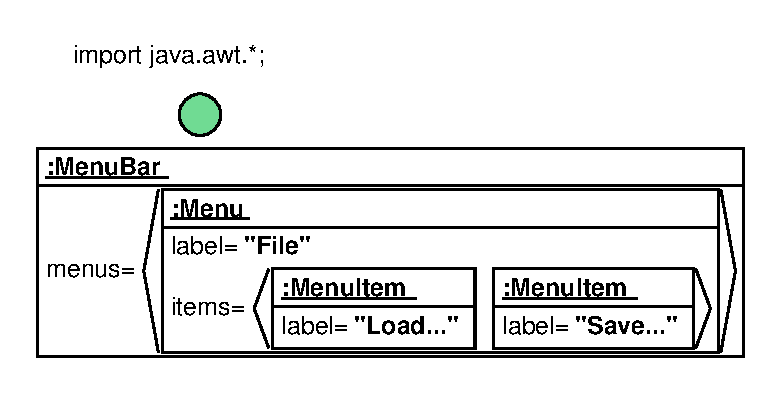
\includegraphics[scale=\netscale]{TokenObjectExample.eps}%
    }
  \caption{\label{fig:TokenObjectExample}An Example of Browsing Token
    Objects in Expanded Tokens Mode}
\end{figure}%

The first compartment specifies a
temporary name of the object (Renew just gives numbers to objects),
followed by a colon (\texttt{:}), followed by this object's class name.
According to UML, the whole string is
underlined to indicate that this is an instance, not the class.
The second compartment is only shown if you click the shutter handle,
a small yellow rectangle with a cross (plus sign) inside.
Otherwise, the available information is indicated by three dots
(\texttt{...}) after the class name.

The second compartment contains a list of all attributes of the token
object and their values, which are basic types or again objects.
Multi-valued attributes (e.g.\ array values or \texttt{Enumeration}s)
are shown as lists in sharp brackets (this part is not quite UML).
After opening the attributes compartment, the handle changes to a
horizontal line (minus sign) and lets you close the compartment again
if you wish to do so.
This way, you can browse the object graph starting at the token
object.
If the value of an attribute happens to be an object that already
appeared in the open part of the object graph, only the temporary name
(number) of that object is display as the attribute's value.
To help you find the original object, you can click on this object
number, and all appearances of this object are highlighted by a red
frame. To get rid of the highlighting, just click on any of the
numbers again.

Figure~\ref{fig:TokenObjectExample} shows an example of a
\texttt{java.awt.MenuBar} object that is being browser as an Expanded
Token. In the example, the menu bar contains one menu \texttt{File}
with two menu item of which the first one is \texttt{Load\dots{}}.
The \texttt{parent} of the first menu item is again the menu, as you
can see by the highlighting. The second menu item is closed.

Renew tries to find attributes of the token object by using Java's
reflection mechanism on fields and \texttt{get}-methods.
Any method without parameters and with a return type which is not
\texttt{void} is regarded a \texttt{get}-method.
In some cases, such methods return volatile (changing) results, but
are only queried once when the token figure is expanded.
This means you should not expect to see changes of a token object
while browsing it!

Renew stores for each place the preferred display mode chosen by
the \texttt{Marking} menu. This means that every new simulation starts
with the display mode chosen for each place, and the display mode is
also saved to disk.
The menu can also be used to change the display mode during run-time.
To do this, either the token figure or the place instance has to be
selected.

\subsubsection{Breakpoints}

Using this attribute, you can request breakpoints for certain
places and transitions. These breakpoints will be established
immediately after the start of the simulation and have exactly
the same effect as a global breakpoint that is set during the
simulation.
In the net drawing, transitions and places with a set
breakpoint attribute are marked by a small red circle in their upper
right corner.
However, the tag is not shown in instance drawings.

Attributed breakpoints, like breakpoints set during the
simulation, will show up in the breakpoint menu while the
simulation is running.
Please see subsection~\ref{subsec:breakpoint}
for a detailed description of the possible breakpoints. Note that you
can set at most one breakpoint for each net element
using this menu command.

Attributed breakpoints are established only when the net drawing is loaded
in the editor at the moment where the compiled net is passed to the
simulation engine.
For the initial drawings (that were used to start the simulation) this is
usually the case.
But if nets are loaded later by the net loader from \texttt{.sns} files
(see Subsection~\ref{subsec:netLoading}), no breakpoints are set.

This behavior is due to the fact that
the responsibility for the creation of breakpoints lies in the
graphical user interface and not in the simulation engine. Since
the breakpoint attribute is dropped when exporting shadow net
systems (see Subsection~\ref{subsec:expshadow}), the 
simulator is not able to establish these breakpoints.

\subsubsection{Set Selection as Icon}
\label{subsubsec:icon}

This feature allows you to assign icons to your nets.
These icons will be displayed during simulation, whenever
a place marking is displayed in \texttt{token} mode
(see subsection~\ref{subsubsec:marking}) and
references an instance of a net
with an icon.

Select exactly one figure, which can be of any type, then select the
menu \texttt{Set Selection as Icon}.
If more than one figure was selected, nothing happens,
but in the case of a single figure, it is assigned as the
net's icon.
When the figure is removed, the net does not have a special icon, so
that references to this net are again displayed as text.
When the figure is or includes a text figure, the string
\texttt{\$ID}, contained anywhere within the text, has a special
meaning: During simulation, \texttt{\$ID} will be replaced by the
index number of the referenced net instance.

You can use net icons as in the following example which can be found
in the samples folder \texttt{icon}.
Remember the Santa Claus example from Section~\ref{sec:channels}?
Imagine you want to visualize the bag and its contents as icons.
Figs~\ref{fig:iconsanta} and \ref{fig:iconbag} show modified versions of the
nets from the Santa Claus example.

\doublenet{iconsanta}{iconbag}

Add an icon to the \texttt{bag} net by drawing an ellipse,
coloring it gray, and drawing a polygon which looks like the closure
of the bag.
Add a text with the string \texttt{BAG \$ID} to the drawing.
\iffalse
Be careful not to connect the text to any other figure (see bug
below).
\fi
Group together all new figures (\texttt{Edit | Group}).
This is necessary, since the icon of a net has to be a single figure.
Now you can select the group and then the menu \texttt{Set Selection
as Icon}.
Note that when you have to \texttt{Ungroup} the icon (e.g.\ to move one
of the included figures individually), this corresponds to removing
the group figure. So, after re-grouping the icon, you have to invoke
the menu again, or the group figure will not be set as the net's icon.

The next step to make an iconized version of the Santa Claus example
is to create a new net, add an image figure with your favorite sweet
(in my case, this is a muffin) and a text figure saying \texttt{\$ID}.
Then again group together the image and the text, select this new
group, and select the menu \texttt{Set Selection as Icon}.
Save this net as \texttt{muffin}.

Now, you can select the net \texttt{iconsanta} and  start a new
simulation. After performing two steps, the running nets may look like
those in Figure~\ref{fig:santabagmuffin}.
Note that the reference to the net \texttt{bag} is now display as the
bag icon with \texttt{\$ID} replaced by the net instance index 1.
Without the icon, the token would have been described as
\texttt{bag[1]}. Also note that the muffins all have different index
numbers, so that you can see to which net they refer.

\begin{figure}[htbp]
  \centerline{%
    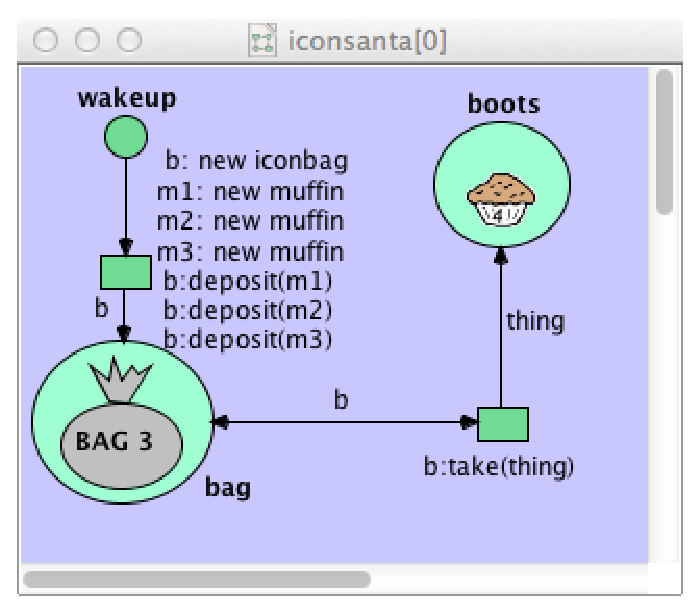
\includegraphics[scale=\screenshotscale]{iconsanta-screenshot2-5}%
    \vspace{1pt}
    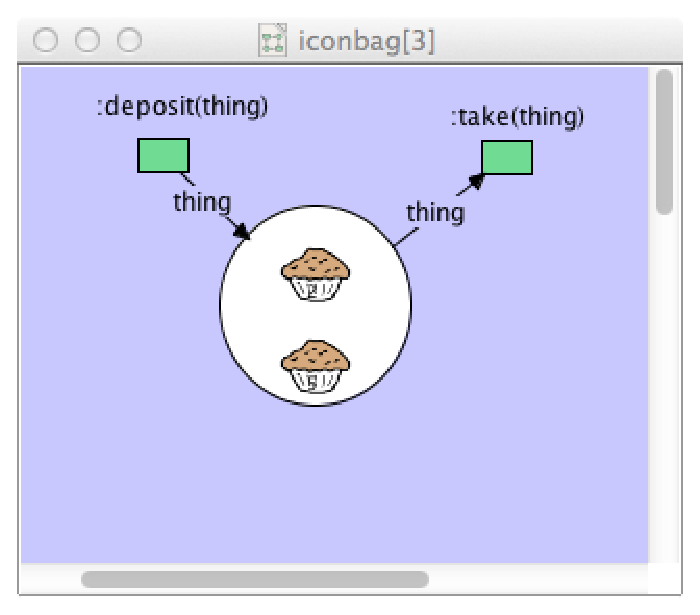
\includegraphics[scale=\screenshotscale]{iconbag-screenshot2-5}%
    }
  \caption{\label{fig:santabagmuffin}The Santa Claus Example with
    Icons During Simulation.}
\end{figure}%


\tip{The background of expanded tokens in instance/simulation drawings is not transparent by default to improve readability. It can be changed to be transparent by setting the property \texttt{de.renew.gui.noTokenBackground}.}

\iffalse
% Bug fixed. Comment probably not needed any longer.
\bug{
  There is a bug when putting connected text into a
  group. Whenever such a group is copied, Renew throws an
  exception. For example in case of a text element in a net icon, you
  have to be careful not to connect this text to the figure,
  because afterward you want to group together the text with the
  figure and Renew will try to copy this group figure during
  simulation.
  Unfortunately, connecting text happens quite easily when you move
  the unconnected text, as a figure below it will become its parent.
  Instead, you should move the figure below, not the text itself, and
  then move the group as a whole later on.
  Another possibility is to select the unconnected text and another
  figure, since when multiple figures are selected, Renew will not
  assign new parents.
}
\fi


\subsubsection{Associate Highlight}

It is not only possible to select the kind of feedback given for
the marking of a place (see Subsection~\ref{subsec:netinstwind}), but
also to specify arbitrary graphical elements to be highlighted
whenever a place is marked or a transition is firing.
Each net element can have at most one highlight figure, but this
figure can be any Renew drawing figure like any rectangle, line, text,
etc., even a group figure.

You can for example draw a StateChart with Renew's drawing
facilities, construct a net which simulates the StateChart's
behavior, and associate figures such that during simulation,
the StateChart is highlighted accordingly.

The first function one needs for dealing with such highlights is to
associate a highlight to a net element such as a place or a
transition.
When the menu \texttt{Associate Highlight} is invoked, exactly two
figures have to be selected, of which one has to be a place or a
transition.%
\footnote{It is even possible to associate another net element as a
highlight, but this is not recommended, as it can lead to confusion.
}
The status line tells you if associating the highlight to the net
element was successful, otherwise displays an error message.

Now, during simulation, the associated figure will be
highlighted exactly when the net element is highlighted.
If the associated figure is invisible, it will be made visible whenever
it is highlighted. If the figure is already visible, its color
will change as a result of the highlighting.

\subsubsection{Select Highlight(s)}

To find the associated highlight figure (see above) to a net element,
select the net element and then this menu.
If the net element does not have any highlight figure, a corresponding
message appears in the status line.
You can also select multiple net elements, and all associated
highlight figures of any one net element of the group will be selected.

\subsubsection{Unassociate Highlight}

Sometimes you also want to get rid of a highlight-association (see
above). Then, select one single net element (place or transition) with
an associated highlight figure and then invoke this menu.
When you associate a net element to a highlight figure, any old
association is automatically canceled.



\subsubsection{Syntax Check}

This menu entry checks the net for syntax errors without
starting a simulation run. Of course, most syntax errors are
immediately reported after the editing of an inscription,
but not all errors are found this way. E.g., multiple uplink
inscriptions cannot be detected immediately. You can also
invoke a syntax check when you have corrected one error,
in order to make sure that no other error remains. It is
always a good idea to keep the nets syntactically
correct at all times.

\iffalse
% The lint checks have been removed to avoid inconsistencies with
% the new formalism model.
\subsubsection{Channel Check}

This menu entry checks for patterns in the synchronous channel
inscriptions that could throw the simulator into an infinite loop.
In these cases, one or more transitions have a downlink and an uplink,
so that a transition can invoke itself through synchronous channels.
There are occasions when this is sensible, but it should only be
used in experimental models.

For productions models you should
make sure that the simulator behaves correctly by running this
check once.
If the check fails, it reports the cyclic dependency of channels
that was found. Removing this problem can cause a substantial
amount of work, because a loop needs to be made explicit
in the net structure.

The check can also fail if a downlink does not have a matching
uplink. That means the offending transition can never fire.
This is usually a misspelled channel name and not a deep problem.

It is not reported as an error when an uplink does not have a matching
downlink, because this simply indicates that some functionality
of a net is not yet needed and it might well be required in the
future. The unmatched uplink might also be needed for a
Java stub as described in Section~\ref{sec:netcall}.


\subsubsection{Name Check}

This menu entry checks for net elements with the same
name within one net. This error is not reported
in the normal syntax check, because there might be occasions
when it is sensible to have a place and a transition that share
the same name, or even two transitions with the same name.
But since a repeated name can indicate a subtle modeling
problem, this check is provided.


\subsubsection{Isolated Node Check}

This menu entry checks for net elements which are not
connected to others.  This error is not reported in the normal syntax
check, because there are situations when isolated net elements might be
reasonable.  Normally, an isolated node indicates a modeling
problem.
\fi

\subsubsection{Layout Check}

This menu entry checks in all loaded drawings whether
textfields overlap by more than 50\%.  Overlap indicates problems in the
clear representation. Also, the situation is detected that a second
inscription is accidentally assigned to an arc and is hidden because of the
overlap.


\subsection{Simulation}
\label{sec:simulation}

This menu controls the execution or simulation of the net system
you created (or loaded).
Before a simulation can be started, all necessary nets must be loaded into
memory (see subsection~\ref{subsec:menuDrawings}).
The drawing window containing the net that is to be
instantiated initially has to be activated.

Refer to Section~\ref{sec:simcontr}, if you want to learn how to
monitor and influence a simulation run
that you have started using this menu.

\subsubsection{Run Simulation}

This function starts or continues a simulation run that continues
automatically until you stop the simulation.
If you want to enforce starting a new simulation run, use
\texttt{Terminate Simulation} (see below) first.
For most net models, it is almost impossible to follow what's going
on in this simulation mode. Its main application is to execute a
net system of which you know that it works.

Some syntax checking is done even while you edit the net (see
Section~\ref{subsubsec:toolInscription}: The Inscription Tool),
but when you try to run a simulation of your reference nets,
the reference net compiler is invoked and
may report further errors (see Section~\ref{sec:errors}).
You have to correct all compiler errors before you can start a simulation
run.

The keyboard shortcut for this function is \texttt{Ctrl+R}.

\subsubsection{Simulation Step}

This menu performs the next simulation step in the active simulation
run or starts a new simulation run if there is no active simulation.

If a simulation is already running in continuous mode, one more step
is executed and then the simulation is paused to be continued in
single-step mode.
Thus, it is possible to switch between continuous and single-step
simulation modes.

The keyboard shortcut for this function is \texttt{Ctrl+I}.

\subsubsection{Simulation Net Step}
This menu entry performs a series of simulation steps in the active
simulation run or starts a new simulation run if there is no active
simulation.
The simulation is paused when an event in the net instance in the current
instance window occurs.%

The keyboard shortcut for this function is \texttt{Ctrl+Shift+I}.

\subsubsection{Halt Simulation}

This menu halts the current simulation run, which has been
started with \texttt{Run Simulation}, or terminates the
search for a possible binding in single step mode.
No further simulation steps are made, but you are free
to resume the simulation with \texttt{Run Simulation} or
\texttt{Simulation Step}.
\bug{There are situations where a net invokes a Java method that
does not terminate. In these cases Renew cannot succeed
in halting the simulation.}

The keyboard shortcut for this function is \texttt{Ctrl+H}.

On Mac OS X systems, \texttt{Cmd+H} is bound system-wide to
hide the application window.  
Therefore, the shortcut key has been changed to \texttt{Shift+Cmd+H}.

\subsubsection{Terminate Simulation}

This menu entry stops the current simulation run (if there is any).
For certain reasons, the simulator can not know if the simulated
net is dead (it could always be re-activated from
outside, see Section~\ref{sec:netcall}), so a simulation only
ends when you invoke this command. When you issue
another simulation command after this command, a new simulation
is automatically started.

All simulation related
windows (net instances, current markings, now also
possible transition bindings) are now automatically closed
when simulation is terminated, since they cannot be used
after simulation anyway.


The keyboard shortcut for this function is \texttt{Ctrl+T}.

\subsubsection{Configure Simulation\dots{}}
\label{subsec:configureSimulation}

This dialog allows to change some simulation
related configuration options.
These options can also be controlled from the command line or
the configuration file \texttt{.renew.properties} (see
section~\ref{subsec:configMethods}).
All options presented in this dialog are evaluated each time a
new simulation is started.
However, the settings in this dialog are not stored
permanently.

The dialog comprises several tabs, each tab groups some
configuration options.
The buttons at the bottom of the dialog affect all tabs.
\begin{description}
\item[\texttt{Apply}] passes the current settings to the plug-in
  system, so that the simulator plug-in can interpret them at the
  next simulation startup. 
\item[\texttt{Update}] refreshes the dialog to display the
  current settings known to the plug-in system. 
  Unless you modify some properties concurrently, you can think
  of this button as a ``revert'' button, that restores the most
  recently applied configuration.
\item[\texttt{Update from simulation}] refreshes the dialog to
  display the configuration of the running simulation, if there
  is any.
  These settings may differ from the current simulator plug-in
  configuration, so you might want to press \texttt{Apply} or
  \texttt{OK} afterward to bring the plug-in configuration back
  in sync with the settings of the running simulation.
\item[\texttt{OK}] applies the current configuration (like
  \texttt{Apply} would do) and closes the dialog.
\item[\texttt{Close}] closes the dialog and discards any setting
  changes (unless they have been applied before).
\end{description}
The tabs provide the following options:

\paragraph{Engine}
The two options \texttt{Sequential mode} and
\texttt{Multiplicity} configure the concurrency of the simulation
engine.
The sequential mode is of interest when you work with a timed
formalism (see section~\ref{sec:timedNets}) or special arc types
(see section~\ref{subsec:sequentialTools}).
Multiple simulators may enhance the performance on multiprocessor
systems.
A sequential mode with multiplicity greater than one is not
sequential because it uses multiple concurrent sequential
simulators.

The settings are equivalent to the
\texttt{de.renew.simulatorMode} property mentioned in
sections~\ref{subsec:concsim} and \ref{subsec:seqmode}.
Just think of the \texttt{Sequential Mode} check box as the sign
of the \texttt{simulatorMode} value (if you enter a minus sign in
the \texttt{Multiplicity} field, it is ignored).

The \texttt{Class reinit mode} setting equivalents the
\texttt{de.renew.classReinit} property explained in
section~\ref{subsec:classReinit}.
It allows you to reload custom classes during development.

The \texttt{Simulation priority} sets the priority of each thread the simulation 
spawns. 
Higher values allow for faster simulations but might result in reduced GUI responsiveness.
The default value of 5 is considered a good tradeoff between speed and gui response time.

\paragraph{Remote Access}
The options provided by this tab find their equivalents in the
remote properties which are explained in
section~\ref{subsec:remoteSetup}.
When you check \texttt{Enable remote access}, the simulation will
be published over Java RMI to allow remote inspection and
simulation control (this feature needs a running RMI registry to
work).
To distinguish multiple simulations on the same registry, you can
assign a \texttt{Public name} to the simulation.
Plug-In developers might be interested in the possibility to
replace the remote \texttt{Server class} by a custom
implementation.
A custom RMI \texttt{Socket factory} can only be supplied at startup,
therefore this property cannot be changed here.

To observe the simulation from a remote editor, use the the
\texttt{Remote server} command explained in
section~\ref{subsec:connectToServer}.

\paragraph{Net path}
This tab allows the manipulation of the \texttt{de.renew.netPath}
property used by the net loader (see
section~\ref{subsec:netLoading}).
On the left, you have a list of path entries, one directory per
line.
The net loader searches the directories in order from top to
bottom.
In the list, you can select one or more entries to manipulate.
On the right, there are five buttons, most of which affect the
selected set of entries.
\begin{description}
\item[\texttt{Add\dots}] opens a dialog where you can enter a new
  path entry.
  The directory should be entered in os-specific syntax.

  If you want to specify a directory relative to the classpath,
  check the appropriate box and make sure that the path does
  \emph{not} start with a slash, backslash, drive letter or what
  else declares a path absolute at your operating system.
\item[\texttt{Edit\dots}] opens a dialog similar to the
  \texttt{Add\dots} dialog for each selected path entry.
\item[\texttt{Move up}] moves all selected entries one line above
  the first selected entry (or to the top of the list, if the
  topmost entry was included in the selection).
\item[\texttt{Move down}] moves all selected entries one line below
  the last selected entry (or to the end of the list, if the
  bottom-most entry was included in the selection).
\item[\texttt{Delete}] removes all selected entries from the list.
\end{description}

\paragraph{Logging}
This tab configures the simulation log traces (see Menu entry ``Show
simulation trace\dots'' below). %~\ref{subsec:loggingPlugin}).
In contrast to other tabs, changes to the settings on this tab take effect
immediately.

It is possible to create additional loggers that focus on net-, transition-
or place-specific parts of the simulation trace.
A click with the right mouse button on the top-level entry of the logger
tree opens a context menu where additional loggers can be added.
The logger name serves as filter criterion.

Each logger can be configured to send its data to one or more appenders.
Depending on the kind of appender, the filtered simulation trace can go to
the console, a file or a trace window (\texttt{GuiAppender)}.
Each appender can be configured with various options.
For example the buffer size (the number of viewable simulation steps) of
the \texttt{GuiAppender} can be adjusted to your needs. 
%% TODO: Detailed description of configuration options.

The textfield \texttt{Layout} is used to customize logger output 
using log4j PatternLayout.

\subsubsection{Remote server\dots{}}
\label{subsec:connectToServer}

Using this menu entry, you can list all net instances of a
Renew simulation server. To be able to do this, a simulator must be running
with remote access enabled as described in
section~\ref{subsec:remoteSetup}.

The dialog comprises two parts:
The upper buttons switch between remote simulations, the lower
part shows a list of net instances.
Initially, the list shows net instances of the local simulation
(if there is a running simulation).

The \texttt{Connect\dots} button displays another dialog which
allows you to connect to a remote simulation server.
You must specify the host on which the \texttt{Server} is running.
The server \texttt{Name} can be left at the default value unless
you specified the \texttt{de.renew.remote.publicName} property on
the server side.

If the connection has been established, the drop-down box at the
top of the \texttt{Remote Renew servers} dialog includes the
remote simulation and the list of net instances is updated.
You can switch between servers by selecting them in the drop-down
box.
The connection stays alive until you press the
\texttt{Disconnect} button, or either Renew application (local or
remote) terminates.

In the net instance list, you can select a net instance and open
it by double-click or by pressing the \texttt{Open} button.
The title of the net instance window shows that it is the
instance of another server.
You can use nearly all the interaction features of local net instance
drawings. All your modifications are executed on the server. Like
local simulation windows, events from the remote simulation
ensure that the drawings will be up-to-date at every time.

\bug{The editor is not able to display two net instances with the
  same name and id.
  It will bring the existing net instance window to front when
  you select a net instance with the same name and id from a
  different simulation.
  To see the other net instance, close the existing net instance
  window.}


\subsubsection{Breakpoints}
\label{subsec:breakpoint}

You can set breakpoints to stop the simulation at a predefined
point of time, which is especially helpful for debugging purposes,
where the simulation might have to run for extended periods
of time, before an interesting situation arises.


The breakpoint menu consists of two sections. The first allows
you to set and clear breakpoints and the second allows you to
view all breakpoints currently set in the simulation.

A breakpoint will stop the search for enabled bindings when running
a simulations. However, the execution of those transitions
that are already firing continues. This is especially important if a
breakpoint is attached to a transition: The transition might still
run to completion while the breakpoint is reported.

That means that you will often want
to attach a breakpoint to an input place of a transition, if you
want to inspect the state of the net before a certain
transition fires. You cannot currently detect a change of enabledness
directly.

\paragraph{Set Breakpoint at Selection.}

Before setting a breakpoint you must select a place or transition
or a group thereof within a net instance window.
You can set a breakpoint either locally or globally.
A local breakpoint will affect exactly the chosen net instance
and will not cause a simulation stop if other net instances
change. A global breakpoint automatically applies to
all net instances, even those that will be created after the breakpoint
is established.

There are a number of different breakpoint types:
\begin{itemize}
\item Default. This is a convenience type that is equivalent to
  a breakpoint on start of firing for transitions and on change
  of marking for places. You can use it if you want to set
  a breakpoint to a place and a transition simultaneously.
\item Firing starts. This breakpoint is triggered
  whenever the transition starts firing. The breakpoint happens just
  after all input tokens have been removed from their places and
  the transition is about to execute its actions.
\item Firing completes. Unlike the previous item, the breakpoint
  occurs at the end of a transition's firing. This is especially
  useful in the case of net stubs, where you want to inspect the
  result of a stub call.
\item Marking changes. Any change of the state of a place is detected here,
  even if the change is simply due to a test arc.
\item Marking changes, ignoring test arcs.
  Here it is required that tokens are actually moved and not merely
  tested.
\item $+1$ token. Only a token deposit triggers this breakpoint.
\item $-1$ token. A token removal must occur before this breakpoint
  is activated.
\item Test status changes. Normal arcs do not
  trigger this breakpoint, but test arcs do.
\end{itemize}
Multiple breakpoint types may be set for a single net element
using this menu.

\paragraph{Clear Breakpoint at Selection.}

A breakpoint is not automatically cleared after it was invoked.
Instead, you must clear breakpoints explicitly.
Having selected the net element that contains a
breakpoint, you can either clear all local breakpoints or
all global breakpoints.

\paragraph{Clear All Breakpoints in Current Simulation.}

This command  will get rid of all breakpoints that were ever set.
This is useful if you have reached a certain desired situation
and want to continue the simulation normally. Alternatively,
you might want to clear all breakpoints that were configured using
the attribute menu, if you require a completely automatic run
once in a while, but not want to loose the information about the standard
breakpoints.

\paragraph{Breakpoint List.}

The second part of the menu allows you to view all breakpoints,
locate the associated net elements, and possibly reset individual
breakpoints.


\subsubsection{Save simulation state\dots{}}

This menu entry saves the current simulation state to a file,
so it can be restored later on by the menu command
\texttt{Load simulation state}.
The saved state also includes all net instances currently
opened in drawings and all compiled nets.
The default extension for Renew simulator state files is
\texttt{.rst}.

Points to be aware of:
\begin{itemize}
\item Saved simulation states will most likely not be compatible
      between different versions of Renew.
\item All custom classes used in the current marking of the net
      must implement the interface \texttt{java.io.Serializable}
      in a sensible way to obtain a complete state file.
\end{itemize}

There are also some minor side effects:
\begin{itemize}
\item This command halts the simulator, because there must not
      occur any changes to the current simulation state while it
      is saved to obtain a consistent state file. You can continue
      the simulation afterward.
\item The binding selection window will be closed, if it is
      open.
\end{itemize}

\subsubsection{Load simulation state\dots{}}

This menu entry loads a simulation state from a file
saved by the menu command \texttt{Save simulation state}
before.
You will then be able to continue the simulation as usual
from the point at which the simulation state was saved.

If all drawings used in the state are loaded, you can use
all simulation control facilities as usual.
However, it is not necessary to have all used drawings open.
If some drawing is missing, the only drawback is that its
net instances will not be displayed in instance drawings.
As a consequence, you will not be able to use the extended
control features described in Section~\ref{sec:simcontr}
for these nets, but the menu commands \texttt{Simulation step}
and \texttt{Run simulation} will still work and
trace events will still be logged.
This holds even if no drawing used by the saved simulation
state is loaded at all.

The mapping from a compiled net contained in the saved state
to an open net drawing is done by the net's name.
This mapping occurs every time when you try to open an
instance drawing for any instance of the net.
If you added to or removed from the net drawing
any transitions or places since the simulation state was
saved, some messages informing you about the problem and
its consequences are printed to the application log.
An instance drawing will still be opened, but it will not
necessarily display the same structure that the compiled net
uses.

Further points to be aware of:
\begin{itemize}
\item If you load a simulation state, any running simulation
      will be terminated and all related windows are closed.
\item If the class reinit mode is selected (see Subsection
      \ref{subsec:classReinit}), custom classes will be
      reloaded while restoring the simulation state.
\item All custom classes used in the saved simulation state
      must be available when restoring the state.
\end{itemize}


\subsubsection{Show simulation trace\dots}
\label{subsec:loggingPlugin}
This menu command opens a window that shows the trace of the
current simulation.
In previous Renew releases, the trace has always been printed to the
console, now you can closely inspect the trace inside the editor.
The shortcut for this command is \texttt{Ctrl+L}

By default, the drop-down list on top of the window provides one simulation
trace that covers the last 20 simulation steps.
You can configure additional traces of different length that focus on
specific net instances, places or transitions using the \texttt{Logging}
tab of the \texttt{Configure simulation} dialog (see above).

A double left mouse button click on a simulation trace entry opens a window
that displays the whole message, using multiple lines if appropriate.  
A right mouse button click opens a context menu that allows you to display
the net template or instance that was involved in the simulation step.
It is also possible to select the individual place or
transition in the net template or instance.

\bug{The mouse actions to inspect a trace entry are not available before
  you have selected any line of the simulation step it belongs to.}

\subsubsection{Formalisms}
\label{subsec:formalismgui}

This submenu configures the current formalism
used during compilation and simulation.
Please note that a running simulation will always stay with the
formalism it has been started with.
To apply the chosen formalism to the simulation, you have to
terminate it and start a new one.

The entries of this menu depend on the set of plug-ins currently installed.
The basic renew distribution includes four formalisms, represented by their
compilers:
\begin{description}
\item[P/T Net Compiler] compiles the net as a simple place-transition net.
  It accepts integer numbers as initial markings and arc weights.
  Capacities are not supported.
\item[Java Net Compiler] encapsulates the reference net formalism with Java
  inscriptions as described in chapter~\ref{ch:reference}.
  However, this compiler does not accept time annotations.
\item[Timed Java Compiler] represents the same formalism as the
  \texttt{Java Net Compiler}, but with additional time annotations as
  explained in section~\ref{sec:timedNets}.
  Nets compiled by this compiler must be executed in a sequential
  simulation.
\item[Bool Net Compiler] compiles nets according to the formalism presented
  in \cite{Langner1998}.
  A bool net is a restricted colored net with exactly one color
  $bool:=\{0, 1\}$ (can also be represented as $\{\mathtt{false},
  \mathtt{true}\}$).
  It accepts one of the propositional logic operators \texttt{and},
  \texttt{or} and \texttt{xor} as transition guard inscriptions.
\end{description}

\subsubsection{Show sequential-only arcs}
\label{subsec:sequentialTools}

This option is available only when the
\texttt{Java Net Compiler} is chosen as current formalism.
Selecting this option adds another toolbar to the editor.
This toolbar comprises two additional arc types (see
section~\ref{subsubsec:toolArc}) which are allowed in
sequential simulations only.
Please note that this option is automatically enabled (although
the menu entry is not visible) when you choose the
\texttt{Timed Java Compiler} as formalism.

For your convenience, the sequential simulation mode (see
sections~\ref{subsec:configureSimulation} and
\ref{subsec:seqmode}) is activated each time you check the box or
choose the \texttt{Timed Java Compiler}.
However, the engine is not switched back to concurrent mode when
you uncheck the box or change to another formalism.


\subsection{Windows}
\label{subsec:menuDrawings}

This menu contains a list of all drawings loaded into memory.
The drawings are classified into \texttt{Nets},
\texttt{Net instances} and \texttt{Token Bags} and appear in
alphabetically sorted submenus.

A drawing can be loaded supplying its file name to Renew as a
command line argument, invoking the \texttt{Open Drawing\dots{}}
menu, or created through the \texttt{New Drawing} menu.
A newly created drawing can be named and any drawing can be
renamed by saving it using the \texttt{Save Drawing as\dots{}} menu.

By selecting a drawing in the \texttt{Windows} menu, its window
is raised and becomes the active drawing window.
In the menu, the name of the active drawing appears checked.

Non-modal tool and attribute dialogues are included in the windows menu in
their own categories.
These windows are raised when the corresponding menu entry is selected,
but there is no effect with respect to the list of active drawings.

\subsection{Additional Top-Level Menus}
\label{sec:additional-top-level}

The menu manager allows for the registration of a menu item by the
plugins under any top-level menu.
%
Additionally, plugins may use a new top-level name.
%
Typical candidates are \emph{Plugins}, \emph{Tools} and
\emph{Application}

The optional plugin \emph{GuiPrompt} offers
its command under the \emph{Plugins} menu. The \emph{NetComponents}
plugin and the optional plugins%
\footnote{All mentioned optional plugins are not part of the release
of Renew. They are provided separately.} \emph{Diagram}, 
\emph{NetDiff} and \emph{Lola} reside under the
\emph{Tools} menu. Since version 2.3 it is also possible to
determine the position of the menu item within the menu. The
\emph{Navigator} plugin extends the \emph{File} menu.

\section{Net Simulations}
\label{sec:simcontr}

During simulation, there may be textual and graphical feedback.
The Log4j framework receives simulation events and can log them
alternatively to the console, a file, the trace window, etc.
In Subsection~\ref{subsec:loggingPlugin}, the graphical configuration dialog
for Log4j is explained.
In a trace of log events, you can see exactly which transitions fired and
which tokens were consumed and produced.
Alternatively, you can view the state of the various net instances graphically
and you can influence the simulation run. 
The following sections describe the means to monitor and control the simulation.


\subsection{Net Instance Windows}\label{subsec:netinstwind}

The graphical feed-back consists of special windows, which contain
instances of your reference nets.
When a simulation run is started,
the first instance of the main reference net that is generated is
displayed in such a net instance window.
As in the simulation log, the name of a net instance
(and thus of its window) is composed of the net's name together
with a numbering in square brackets, e.g.\ \texttt{myNet[1]}.
Net instance windows can also be recognized by their special
background color (something bluish/purple), so they cannot
be confused with the windows where the nets are edited.
In a net instance window, you cannot edit the net, you cannot
even select net elements. The net is in a ``background layer'',
and only simulation relevant objects are selectable, like
current markings of places and transition instances.
Places in net instance windows are annotated with the number of
tokens they contain (if any).
If you double-click on a marking the containing place will be selected.
If you right-click on such a marking, the marking will switch between 
the number of tokens and the tokens in a string representation.
If you right-click on the containing place, another window appears,
containing detailed information about the tokens.

You can display the contents of the current marking directly
inside the net instance window.
This is extremely useful when a place
contains only few tokens (or even only one). This also helps
to control the number of windows, which could become very
large using Renew.
To switch between the simple (cardinality of the
multiset) and the token display of a place marking, just
right-click it.
The expanded display behaves exactly like the contents of a
current marking window, which is described in the following
section.
Tokens in markings are always displayed with a white, opaque
background.
This increases the readability of markings.  


\subsection{Current Marking Windows}

A current marking window shows the name of the corresponding place
(net instance name dot place name, e.g.\ \texttt{myNet[1].myPlace})
in its window title bar.
If the token list does not fit into the current marking window,
the scroll bars can be used.
For each different token value in the multiset, a current marking
window shows the multiplicity (if different from one) and
the value itself.
%The token value is usually displayed as some String, using the Java method
%\texttt{toString()}, which is supported by every Object.
The Expanded Tokens mode described in
Subsection~\ref{subsubsec:marking} is now the default mode for
current marking windows (if the FS plug-in is installed).

There is a special function to gain access to other net instances.
If a token's value is or contains a net instance, a blue frame appears
around the name of the net instance.
If you click inside that frame, a new net instance window for
that net instance is opened or the corresponding net instance
window is activated, if it already existed.
This also works for net references contained within
a tuple, or even within a nested tuple.
Using the Expanded Tokens mode, this also works for net references
contained within a list or inside any other Java object

\tip{You can open a net instance window,
double click all places you want to ``watch'' and close
the net instance window again. This helps to focus on the
state information you really want to see.
}

%Another feature since 1.1 is that when you double-click a token which
%is a reference to some \texttt{java.awt.Window} object (like a
%\texttt{java.awt.Frame}), this window is raised to the top.

\subsection{Simulation Control}

In a concurrent system, many transitions can be activated at
once.
Normally, the simulation engine decides which of these
transitions actually fires when the next simulation step
is executed.
For debugging and testing, it can be very convenient for
you to take care of this decision. Of course, this only
makes sense when the simulation is performed step by step
(see below).

Interactive simulation is possible.
You can force a specific enabled transition to fire in two ways:
\begin{itemize}
\item Right-click the transition. Here, the simulation engine
  still decides nondeterministically about the variable bindings.
\item Double-click the transition. Then, the so-called
  binding selection window is shown and switched to the
  transition you double-clicked. The title of the window
  says ``{\em transition-name\/}'s possible bindings'', where
  {\em transition-name\/} is the full name (name of the net
  instance-dot-transition-name) of the transition.

  In the top part of the window a single binding is described.
  Each transition instance that participates in this binding
  is shown on a single line, listing
  those variables that are already bound.
  See Section~\ref{sec:channels} for an explanation why multiple
  transition instances might participate in a single firing.
  At the bottom of the window there is a list of all possible
  bindings, where each binding is displayed in a single row.

  When you press the \texttt{Fire} button, the binding of the
  entry which is currently selected will be used in the firing.
  This window should be automatically updated whenever the net's
  marking changes. Use the \texttt{Update} button, if the
  automatic update fails, and make sure to report this as a bug.
  \texttt{Close} hides the transition binding window.
\end{itemize}
%
If the clicked transition is not activated, the status line
of the Renew window tells you so and nothing else is going to
happen.

There are situations where a transition cannot be fired
manually, although it is activated. This is the case for
all transitions with an uplink. Since a transition with an
uplink is waiting for a synchronization request from any
other transition with the corresponding downlink,
Renew cannot find such ``backward'' activations.
You have to fire the transition with the downlink instead.

You should experiment with the simulation mode using some of the
sample net systems first. Then, try to get your own reference nets
to run and enjoy the simulation!


\section{Simulation Server}
\label{sec:simulationServer}

Renew supports client/server simulations via RMI. You can set up
a simulation as a Java VM of its own. You are then able to connect
both locally and remotely, as long as the connection between the
computers allows RMI calls (e.g.\ no firewall blocks them).

As a consequence of the decomposition of Renew
into several plug-ins, any simulation can be published over RMI.
You just need to set the appropriate properties as explained in
section~\ref{subsec:remoteSetup} or use the \texttt{Configure 
Simulation} dialog (see
section~\ref{subsec:configureSimulation}).
Therefore, this section does not focus on the configuration of a
remote simulation, it just describes how to set up a simulation
without using the editor's graphical user interface.

To do this, you have to export all required nets as a shadow
net system first (see~\ref{subsec:expshadow} for details). Whenever you make
changes to any net of this net system, you have to generate the
shadow net system again and start a new server with it.

Now you are ready to start the server itself, by issuing the
following command to the Renew plug-in system:
\begin{lstlisting}[style=xnonfloating]
  startsimulation <net system> <primary net> [-i]
\end{lstlisting}
The parameters to this command have the following meaning:
\begin{description}
        \item[\texttt{\mbox{net system}}:]
                The \texttt{.sns} file, as generated in the step above.
        \item[\texttt{\mbox{primary net}}:]
                The name of the net, of which a net instance shall be opened when the simulation starts. Using the regular GUI, this equals the selecting of a net before starting the simulation.
        \item[\texttt{\mbox{-i}}:] If you set this optional
                flag, then the simulation is initialized only, that
                is, the primary net instance is opened, but the
                simulation is not started automatically.
\end{description}

As mentioned in section~\ref{sec:plugins}, the command can be passed
to the plug-in system by several means.
For example, to start a remotely accessible simulation with net
\texttt{systemnet} out of the net system \texttt{allnets.sns} direct
from the java command line, you will have to issue the following
command (in Unix syntax, the \verb:\: indicates that the printed lines
should be entered as one line):
\begin{lstlisting}[style=xnonfloating]
  java -Dde.renew.remote.enable=true -jar renew§\renewversion§/loader.jar startsimulation allnets.sns systemnet
\end{lstlisting}
If you need a special simulation mode or any other Renew property to
be configured, you can add multiple \texttt{-D} options or use one of
the other configuration methods mentioned in
section~\ref{subsec:configMethods}.

A simulation started by the \texttt{startsimulation} command
differs slightly from a simulation started by the editor:
The net loader does not look for \texttt{.rnw} files, it loads
nets from \texttt{.sns} files only.

If you want to experiment with properties and commands, or if you need
to pause and run the simulation interactively, you should install the
Console plug-in (see section~\ref{subsec:consolePlugin}).
When a simulation is running, several commands can be entered at the
prompt to control the simulation.
These commands provide the same functionality as the menu entries
listed in section~\ref{sec:simulation}.
In fact, if you use the Console plug-in in combination with the
graphical editor, both command sets (menu and console) control the
same simulation.
The console commands are:
\begin{description}
\item[\texttt{\mbox{simulation run}}:]
  Resumes a stopped simulation.
  If the \texttt{-i} option was appended to the
  \texttt{startsimulation} command, this command starts
  the simulation.
\item[\texttt{\mbox{simulation step}}:]
  Executes another simulation step. 
  If the \texttt{-i} option was appended to the
  \texttt{startsimulation} command, this command executes
  the first simulation step.
\item[\texttt{\mbox{simulation stop}}:]    
  Halts the simulation, but does not abandon it, despite of
  the \texttt{term} command. The \texttt{run} command
  continues it.
  This is equivalent to the menu entry \texttt{Halt simulation}.
\item[\texttt{\mbox{simulation term}}:]
  Ends and abandons the current simulation. 
  This may result in termination of the plug-in system
  (see section~\ref{subsec:systemExit}).
\item[\texttt{\mbox{simulation help}}:]
  Shows a short help for all available simulation commands.
\end{description}


\section{Error Handling}
\label{sec:errors}

Renew helps you to maintain a syntactically correct model
by making an immediate syntax check whenever an inscription
has been changed. Additionally, a syntax check is done
before the first simulation step of a model.
The simulation will not start if there is any error in any net.

If an error is detected, an error window is opened,
which displays the error message. At the bottom of the window
is a button labeled \texttt{select}. Pressing this button
selects the offending net element or net elements and
raises the corresponding drawing. If the error originates
from a text figure, that figure is edited with the corresponding text edit
tool. The cursor is automatically positioned close to the
point where Renew detected the error. For more information on editing see
Section~\ref{subsubsec:toolConnectedText}: The Text Tool.

Renew displays exactly one error at a time. If a second error is
found, the old error message will be discarded and the
new error message will be displayed in the error window.

Some errors are not reported at the place where they
originate. E.g., if you are using a declaration figure,
an undefined variable is detected where
it is used, but the missing definition has to be
added to declaration node. Similar effects might happen
due to missing import statements. This is unavoidable, because
Renew cannot tell an undeclared variable from a misspelled
variable.

\newtwodotfive{
For some errors Renew provides a Quick Fix feature, which is described in the following section. }
Other errors and possible solutions are described in the subsequent sections.

\subsection{Quick Fix}

The Quick Fix feature improves the reporting of syntax errors by providing suitable proposals for remedies and their automatic realization.

For errors of type \emph{No such constructor/field/method},
proposals for correct constructors, fields or methods are provided by
the syntax check. If a constructor with the wrong number or types of
arguments is entered, a list of existing constructor signatures is
provided. If a non-existing field name for a class or an object is
entered, a list of all known field names is provided. If a
non-existing method is entered, a list of known method signatures
where the method name is prefixed by the erroneous method name is
provided. If the method name \texttt{\_()} is entered, a list of all
known methods is provided. 
For errors of type \emph{No such variable}, type proposals are provided.

By double-clicking on one of the proposals or selecting and pressing the \texttt{apply} button, you can apply the proposed fix for the reported error. The Quick Fix changes the erroneous method/field name or constructor into the selected one or declares the variable in the declaration note. It can also automatically add import statements for unambiguous types (requires full qualified class names).  

\subsection{Parser Error Messages}

If the expression parser detects a syntax error,
it will report something like:
\begin{lstlisting}[style=xnonfloating]
Encountered "do" at line 1, column 3.
Was expecting one of:
    "new" ...
    <IDENTIFIER> ...
\end{lstlisting}
This gives at least a hint where the syntax error
originated and which context the parser expected.
In our case the inscription \texttt{a:do()}
was reported, because \texttt{do} is a keyword that
must not be used as a channel name.


\subsection{Early Error Messages}

These errors are determined during the immediate
syntax check following each text edit.

\subsubsection{Bad method call or no such method}

Typically you entered two pairs of parentheses
instead of one. Possibly a class name was mistaken
for a method call. Maybe a name was misspelled?

\subsubsection{Boolean expression expected}

An expression following the keyword \texttt{guard}
must be boolean. Maybe you wrote \texttt{guard x=y}, but
meant \texttt{guard x==y}?

\subsubsection{Cannot cast \dots}

An explicit cast was requested, but this cast
is forbidden by the Java typing rules.
Renew determined at compile time that this cast
can never succeed.

\subsubsection{Cannot convert \dots}

The Java type system does not support a conversion that would
be necessary at this point of the statement.

\subsubsection{Cannot make static call to instance method}

An instance method cannot be accessed statically
via the class name. A concrete reference must be provided.
Maybe the wrong method was called?

\subsubsection{Enumerable type expected}

The operator requested at the point of the error
can act only on enumerable types, but not on
floating point numbers.

\subsubsection{Expression of net instance type expected}

For a downlink expression, the expression before the colon must
denote a net instance. E.g.\ it is an error, if in \texttt{x:ch()} the
variable \texttt{x} is of type \texttt{String}.
Maybe you have to use a cast?

\subsubsection{Expression of type void not allowed here}

An expression of void type was encountered in the middle
of an expression where its result is supposed to be
processed further, e.g.\ by an operator or as an argument
to a method call. Maybe you called the wrong method?

\subsubsection{Integral type expected}

The operator requested at the point of the error
can act only on integral types, but not on
floating point numbers or booleans.

\subsubsection{Invalid left hand side of assignment}

In an \texttt{action} inscription, only variables, fields,
and array elements can occur on the left hand side of an equation.
Maybe this expression should not be an action?

\subsubsection{Multiple constructors match}

A constructor call was specified, but from the types of the
arguments it is not clear which constructor
is supposed to be called.
There are overloaded constructors, but none of
them seems to be better suited than the others.
Maybe you should use casts to indicate the intended constructor?

\subsubsection{Multiple methods match}

A method call was specified, but from the types of the
arguments it is not clear which method
is supposed to be called.
There are overloaded methods, but none of
them seems to be better suited than the others.
Maybe you should use casts to indicate the intended method?

\subsubsection{No such class}

The compiler could not find a class that matches a given class
name, but it is quite sure that a class name has to occur here.
Maybe you misspelled the class name? Maybe you forgot an import
statement in the declaration node?

\subsubsection{No such class or variable}

The meaning of a name could not be determined at all.
Maybe the name was misspelled?
Maybe a declaration or an import statement is missing?

\subsubsection{No such constructor}

A matching constructor could not be found. Maybe the
parameters are in the wrong order? Maybe the number of
parameters is not correct? Maybe the requested constructor
is not public?

\subsubsection{No such field}

A matching field could not be found.
Maybe the name was misspelled?
Maybe the requested field is not public?

\subsubsection{No such method}

A matching method could not be found.
Maybe the name was misspelled? Maybe the
parameters are in the wrong order? Maybe the number of
parameters is not correct? Maybe the requested method
is not public?

\subsubsection{No such variable}

A name that supposedly denotes a variable could not be
found in the declarations. Maybe the name was misspelled?
Maybe a declaration is missing?

\subsubsection{Not an array}

Only expressions of an array type can be postfixed with
an indexing argument in square brackets.

\subsubsection{Numeric type expected}

A boolean expression was used in a context where
only numeric expressions are allowed, possibly
after a unary numeric operator.

\subsubsection{Operator types do not match}

No appropriate version of the operator could
be found that matches both the left and the right hand
expression type, although both expression would be valid
individually.

\subsubsection{Primitive type expected}

Most operators can act only on values of primitive type,
but the compiler detected an object type.

\subsubsection{Type mismatch in assignment}

An equality specification could not be implemented, because
the types of both sides are incompatible. One type must be
subtype of the other type or the types must be identical.

\subsubsection{Variable must be assignable from
\texttt{de.renew.net.NetInstance}}

The variable to which a new net is assigned must
be of type \texttt{NetInstance}, i.e.\ of
exactly that type, of type \texttt{java.lang.Object}, or untyped.
E.g.\ it is an error, if in \texttt{x:new net} the
variable \texttt{x} is of type \texttt{java.lang.String}.
Maybe you have to use an intermediate variable of the proper
type and perform a cast later?

\subsubsection{Variable name expected}

The identifier to which a new net is assigned must denote
a variable. E.g.\ it is an error, if in \texttt{x:new net} the
identifier \texttt{x} is a class name.

\subsubsection{Cannot clear untyped place using typed variable}

A clear arc is inscribed with a variable that is typed.
The arc is supposed to clear an untyped place. Because it
cannot be safely assumed that all tokens in the place will have
the correct type, it might not be possible to clear the
place entirely. Consider declaring the variable that
is inscribed to the arc.

\subsubsection{Cannot losslessly convert \dots}

A typed place must hold only values of the given type.
Hence the type of an output arc expression must be
a subtype of the corresponding place type. The type
of an input arc expression is allowed to be
a subtype or a supertype, but it is not allowed
that the type is completely unrelated.

Maybe you were confused by the slight variations
of the typing rules compared to Java? Have a look at
Subsection~\ref{subsec:types}.

\subsubsection{Cannot use void expressions as arc inscriptions}

Void expressions do not compute a value. If you use
such an expression, typically a method call, as
an arc inscription, the simulator cannot determine
which kind of token to move.

\subsubsection{Class \dots\ imported twice}

In a declaration node there were two import statements
that made the same unqualified name well-known, e.g.,
\texttt{import java.lang.Double} and also
\texttt{import some.where.else.Double}.
Remove one import statement and use the fully qualified
class name for that class.

\subsubsection{Detected two nets with the same name}

The simulator must resolve textual references to nets
by net names, hence it is not allowed for two nets to
carry the same name. Maybe you have opened the same net twice?
Maybe you have created new nets, which have the name
\texttt{untitled} by default, and you have not saved
the nets yet?

\subsubsection{Flexible arcs must be inscribed}

A flexible arc is not equipped with an inscription.
Flexible arcs are supposed to move a variable amount
of tokens to or from a place, but this arc does not
depend on any variables and lacks the required variability.
Maybe you did not yet specify an inscription?
Maybe the inscription is attached to the wrong net element?
Maybe you want to use an ordinary arc instead?

\subsubsection{For non-array inscriptions the place must be untyped}

An inscription of a flexible arc is given as
a list or a vector or an enumeration, but the output place is typed.
The resulting restriction on the element types could not be verified.
Maybe it is possible to use an array inscription?
Maybe the place should not be typed?

\subsubsection{Incorrect type for flexible arc inscription}

An inscription of a flexible arc is expected to evaluate to
an array or a list or a vector.
It is only allowed to use enumerations on output arcs,
because the elements might have to be accessed multiple times
in the case of input arcs.
Use an inscriptions that is correctly typed.
Maybe the compiler determined the type \texttt{java.lang.Object},
but it is known that only arrays will result from the expression.
In that case, use an explicit cast to indicate this fact.

\subsubsection{Null not allowed for flexible arcs.}

An inscription of a flexible arc is expected to evaluate to
and array or a list. The compiler was able to determine that
the given expression will always evaluate to \texttt{null}.
Maybe the inscription is attached to the wrong net element?
Maybe the arc was not intended to be a flexible arc?

\subsubsection{Only one declaration node is allowed}

You have two or more declaration nodes in your net drawing.
In general, the simulator cannot determine in which
order multiple declaration nodes should be processed,
hence this is not allowed.
Maybe a declaration node was duplicated unintentionally?
Maybe you want to merge the nodes into one node?

\subsubsection{Output arc expression for typed place must be typed}

A typed place must only hold values of the given type.
An untyped output arc is not guaranteed to deliver an
appropriate value, so this might lead to potential problems.
Maybe you want to type your variables? Maybe you
want to remove the typing of the place?

\subsubsection{Place is typed more than once}

At most one type name can be inscribed to a place.
Multiple types are not allowed, even if they are identical.
Maybe a type was duplicated unintentionally?

\subsubsection{Time annotations are not allowed}

The compiler detected an annotation of the form
\texttt{...@...}, but the current compiler cannot handle
such inscriptions, which require a special net formalism.
You should switch to the \texttt{Timed Java Compiler} (see
Subsection~\ref{subsec:formalismgui}).

\subsubsection{Transition has more than one uplink}

At most one uplink can be inscribed to a transition.
Maybe an uplink was duplicated unintentionally?
Maybe one uplink has to be a downlink?

\subsubsection{Unknown net}

In a creation expression an unknown net name occurred.
Maybe the name is misspelled? Maybe you have not opened the
net in question?

\subsubsection{Variable \dots\ declared twice}

In a declaration node there were two declarations
of the same variable. Remove one variable declaration.

\subsubsection{Variable \dots\ is named identically to an imported class}

In a declaration node there was a variable declaration and
an import statement that referenced the same symbol, e.g.,
\texttt{import some.where.Name} and \texttt{String Name}.
This error is rare, because by convention class names should start
with an upper case letter and variable names should start with
a lower case letter. You should probably rename the variable.

\subsubsection{Variable of array type expected}

If a clear arc is inscribed with a typed variable,
that variable should have an array type, so that
the set of all tokens can be bound to the variable
in the form of an array. You should check whether the
correct variable is used and whether the variable is correctly
typed.


\subsection{Late Error Messages}

Here we discuss the error message that is not reported
during the immediate check, but only during the complete
check before the simulation.


\subsubsection{Unsupported arc type}

An arc of the net was of an illegal type, i.e., the
current net formalism does not support it. This can only
happen when you execute a net with a net formalism that is incompatible
with the net formalism that was used to draw the net.
Maybe you should restart Renew with another net formalism?


% Local Variables:
% mode: latex
% TeX-master:"renew.tex"
% End:

% LocalWords:  Petri unary boolean subclasses instanceof Prolog tuple
% LocalWords:  runtime tuples formalisms workflow uplink downlink
% LocalWords:  untyped subtype supertype booleans multiset selectable
% LocalWords:  cardinality breakpoint appender viewable classpath
% LocalWords:  appenders
